\newif\ifglobal
%%%%%%%%%%%%%%%%%%%%%%%
%%% Compile to view %%%
%%%%%%%%%%%%%%%%%%%%%%%

%%%%%%%%%%%%%%%%%%%%%%%%%%%%%%%%%%%%%%%%%%%%%%%%%%%
%%% Readme:                                     %%%
%%% https://www.overleaf.com/read/bwdjvfjksvjy/ %%%
%%%%%%%%%%%%%%%%%%%%%%%%%%%%%%%%%%%%%%%%%%%%%%%%%%%

% >>> M?: marks a module setting number or important notice

% >>> M4: Set {./relative-path} to external files for this module <<<
\def \modulefiles {./10-PERMCTRL}
% To add an external file, use:
% (Replace '---' with actual filename)
% '\input{\modulefiles/tables/---.tex}' for tables
% '\includegraphics{\modulefiles/figures/---}' for figures
% '\subfile{\modulefiles/---}' for register files

% >>> M1: This module is in global project? <<<
% 'YES' - uncomment; 'NO' - comment out
\globaltrue

\ifglobal
    \documentclass[main\_\_EN.tex]{subfiles}

\else
    \documentclass[openany, 10pt]{book}

    % >>> M2: In ./00-shared/preamble-trm-module, also find
    %         settings for visibility of todo notes, watermark <<<
    \usepackage{preamble-trm-module}

    % >>> M3: Temporary labels in English,
    %         you can add your own labels there <<<
    \myexternaldocument{./00-shared/temp-labels-en}

\fi %\ifglobal


\setcounter{secnumdepth}{4}

% >>> M5: If this module needs any updates in
% './00-shared/preamble-trm-module.sty'
% (include additional package, etc.), contact your module PM
% or create the file './00-shared/changelog.tex' make the
% necessary updates yourself and document them in this file <<<


\begin{document}


% Sets language into which pre-defined bits of text are translated
\selectlanguage{english}

% Do not delete this block
\ifglobal
% Add the following front matter if
% this module is outside of global project
\else
    \InputIfFileExists{readme}{}{}
    {\let\clearpage\relax \listoftodos}
    \tableofcontents
    \listoftables
    \listoffigures
\fi


%%%%%%%%%%%%%%%%%%%%%%%%%
%%% TRM Module Begins %%%
%%%%%%%%%%%%%%%%%%%%%%%%%

\hypertarget{permctrl}{}
\chapter{Permission Control (PMS)}
\label{mod:permctrl}
\section{Overview}

\chipname{} is specially designed for flexible access management to internal memory, external memory, and all peripherals. Once configured, CPU can only access a particular slave device according to the configured permission, thus protecting the slave device from unauthorized access (read, write, or instruction execution).

In addition, \chipname{} has integrated a World Controller, which when enabled can be used along with Permission Controller to allocate the chip's hardware and software resource into Secure World (World0) and Non-secure World (World1), and can switch the CPU between running from the Secure World or Non-secure World. For details, please refer to \ref{mod:wctrl} \textit{\nameref{mod:wctrl}}.

This chapter mainly describes the access management to different internal memory, external memory and peripherals.

\section{Features}

\chipname{}'s Permission Control module supports:
\begin{itemize}
    \item Independent access management for the Secure World and Non-secure World.
    \item Independent access management to internal memory, including
    \begin{itemize}
        \item CPU access to internal memory
        \item Allocate internal memory as CPU Trace
        \item GDMA access to internal memory
    \end{itemize}
    \item Independent access management to external memory, including
    \begin{itemize}
        \item SPI1 access to external memory
        \item GDMA access to external memory
        \item CACHE access to external memory
    \end{itemize}
    \item Independent access management to peripheral regions, including
    \begin{itemize}
        \item CPU access to peripheral regions
        \item Interrupt upon unsupported access alignment
    \end{itemize}
    \item Address splitting for more flexible access management
    \item Interrupt upon unauthorized access
    \item Register locks to secure the integrity of Permission Control related registers
    \item Protection to secure the integrity of CPU's VECBASE registers
\end{itemize}
\section{Internal Memory}

\chipname{} has the following types of internal memory:
\begin{itemize}
    \item ROM: 384 KB in total, including 256 KB Internal ROM0 and 128 KB Internal ROM1
    \item SRAM: 512 KB in total, including 32 KB Internal SRAM0, 416 KB Internal SRAM1, and 64 KB Internal SRAM2
    \item RTC FAST Memory: 8 KB in total, which can be split into two regions with independent permission configuration
    \item RTC SLOW Memory: 8 KB in total, which can be further split into two regions each with independent permission configuration
\end{itemize}

This section describes how to configure the permission to each types of \chipname{}'s internal memory.

\subsection{ROM}\label{sec:permctrl-PC-for-ROM}

\chipname{}'s ROM can be accessed by CPU's instruction bus (IBUS) and data bus (DBUS) when configured. Note:
\begin{itemize}
    \item Permission for Secure World and Non-secure World can be configured independently.
    \item Once configured, the permission applies for both CPU0 and CPU1.
\end{itemize}

\subsubsection{Address}

\chipname{}'s ROM address and the address ranges accessible for IBUS and DBUS respectively are listed in Table  \ref{tab:permctrl-ROM_block_address}.

\begin{table}[H]
    \centering
    \caption{ROM Address}
    \label{tab:permctrl-ROM_block_address}

    \begin{tabular}{|*{5}{c|} }
    \hline
        \rowcolor{lightgray}
         & \multicolumn{2}{c|}{\textbf{IBUS Address}} & \multicolumn{2}{c|}{\textbf{DBUS Address}} \\\cline{2-5}
        \rowcolor{lightgray}
        \multirow{-2}*{\textbf{ROM}} & \textbf{Starting Address} & \textbf{Ending Address} & \textbf{Starting Address} & \textbf{Ending Address} \\\hline

        % table contents
        Internal ROM0  & 0x{}4000\_0000 & 0x{}4003\_FFFF & - & - \\\hline
        Internal ROM1  & 0x{}4004\_0000 & 0x{}4005\_FFFF & 0x{}3FF0\_0000 & 0x{}3FF1\_FFFF \\\hline
        \end{tabular}
    \end{table}

\subsubsection{Access Configuration}

\chipname{} uses the registers listed in Table  \ref{tab:permctrl-rom_permconfig} to configure the instruction execution (X), write (W) and read (R) accesses of CPU's IBUS and DBUS, from the Secure World and Non-secure World, to ROM:

\begin{table}[H]
    \centering
    \caption{Access Configuration to ROM}
    \label{tab:permctrl-rom_permconfig}
    \begin{threeparttable}
    \begin{tabular}{|l|l|l|l|}
        \hline
        \rowcolor{lightgray}
        \textbf{Bus} & \textbf{From World} & \textbf{Configuration Registers\tnote{A}}                         & \textbf{Access} \\ \hline
                     & Secure World      & \hyperref[regdesc:PMSCOREXIRAM0PMSCONSTRAIN2REG]{PMS\_CORE\_X\_IRAM0\_PMS\_CONSTRAIN\_2\_REG   {[}20:18{]}}\tnote{B} & X/W/R           \\ \cline{2-4}
        \multirow{-2}{*}{IBUS} & Non-secure World & \hyperref[regdesc:PMSCOREXIRAM0PMSCONSTRAIN1REG]{PMS\_CORE\_X\_IRAM0\_PMS\_CONSTRAIN\_1\_REG {[}20:18{]}}    & X/W/R \\ \hline
                     & Secure World      & \hyperref[regdesc:PMSCOREXDRAM0PMSCONSTRAIN1REG]{PMS\_CORE\_X\_DRAM0\_PMS\_CONSTRAIN\_1\_REG   {[}25:24{]}}\tnote{C} & W/R             \\ \cline{2-4}
        \multirow{-2}{*}{DBUS} & Non-secure World & \hyperref[regdesc:PMSCOREXDRAM0PMSCONSTRAIN1REG]{PMS\_CORE\_X\_DRAM0\_PMS\_CONSTRAIN\_1\_REG   {[}27:26{]}} & W/R   \\ \hline
        \end{tabular}
        \begin{tablenotes}
        \item[A] 1: with access; 0: without access
        \item[B] For example, configuring this field to 0b101 indicates CPU's IBUS is granted with instruction execution and read accesses but not write access to ROM from the Secure World.
        \item[C] For example, configuring this field to 0b01 indicates CPU's DBUS is granted with read access but not write access to ROM from the Secure World.
        \end{tablenotes}
     \end{threeparttable}
    \end{table}

\subsection{SRAM}

\chipname{}'s SRAM can be accessed by CPU's instruction bus (IBUS) and data bus (DBUS) when configured. Note:
\begin{itemize}
    \item Permission for Secure World and Non-secure World can be configured independently.
    \item Once configured, the configuration applies for both CPU0 and CPU1.
\end{itemize}

\subsubsection{Address}

\chipname{}'s SRAM address and the address ranges accessible for IBUS and DBUS respectively are listed in Table  \ref{tab:permctrl-SRAM_block_address}.

\begin{table}[H]
    \centering
    \caption{SRAM Address}
    \label{tab:permctrl-SRAM_block_address}
    \begin{tabular}{ |*{6}{c|}}
    \hline
        \rowcolor{lightgray}
        & & \multicolumn{2}{c|}{\textbf{IBUS Address}} & \multicolumn{2}{c|}{\textbf{DBUS Address}} \\\cline{3-6}
        \rowcolor{lightgray}
        \multirow{-2}*{\textbf{SRAM}} & \multirow{-2}*{\textbf{Block}} & \textbf{Starting Address} & \textbf{Ending Address} & \textbf{Starting Address} & \textbf{Ending Address} \\\hline
        % table contents
        \multirow{2}*{Internal SRAM0}  & Block0 & 0x{}4037\_0000 & 0x{}4037\_3FFF & - & - \\\cline{2-6}
                                    & Block1 & 0x{}4037\_4000 & 0x{}4037\_7FFF & - & - \\\hline
    \multirow{7}*{Internal SRAM1}  & Block2 & 0x{}4037\_8000 & 0x{}4037\_FFFF & 0x{}3FC8\_8000 & 0x{}3FC8\_FFFF \\\cline{2-6}
                                    & Block3 & 0x{}4038\_0000 & 0x{}4038\_FFFF & 0x{}3FC9\_0000 & 0x{}3FC9\_FFFF \\\cline{2-6}
                                    & Block4 & 0x{}4039\_0000 & 0x{}4039\_FFFF & 0x{}3FCA\_0000 & 0x{}3FCA\_FFFF \\\cline{2-6}
                                    & Block5 & 0x{}403A\_0000 & 0x{}403A\_FFFF & 0x{}3FCB\_0000 & 0x{}3FCB\_FFFF \\\cline{2-6}
                                    & Block6 & 0x{}403B\_0000 & 0x{}403B\_FFFF & 0x{}3FCC\_0000 & 0x{}3FCC\_FFFF \\\cline{2-6}
                                    & Block7 & 0x{}403C\_0000 & 0x{}403C\_FFFF & 0x{}3FCD\_0000 & 0x{}3FCD\_FFFF \\\cline{2-6}
                                    & Block8 & 0x{}403D\_0000 & 0x{}403D\_FFFF & 0x{}3FCE\_0000 & 0x{}3FCE\_FFFF \\\hline
    \multirow{2}*{Internal SRAM 2}  & Block9 & - & - & 0x{}3FCF\_0000 & 0x{}3FCF\_7FFF \\\cline{2-6}
                                    & Block10 & - & - & 0x{}3FCF\_8000 & 0x{}3FCF\_FFFF \\\hline
        \end{tabular}
    \end{table}

Here, we will first introduce how to configure the permission to Internal SRAM0, Internal SRAM1, and Internal SRAM2, and also how to configure the Internal SRAM1 as CPU Trace memory.

\subsubsection{Internal SRAM0 Access Configuration}\label{sec:permctrl_sram0}

\chipname{}'s Internal SRAM0 includes Block0 and Block1 (see details in Table \ref{tab:permctrl-SRAM_block_address}) and can be allocated to either CPU or ICACHE.

Note that once configured, the configuration applies for both CPU0 and CPU1.

\chipname{} uses the register described in Table \ref{tab:permctrl-sram0_accessconfig} to allocate the SRAM0 to either CPU or ICACHE:

\begin{table}[H]
    \centering
    \caption{Internal SRAM0 Usage Configuration}
    \label{tab:permctrl-sram0_accessconfig}
    \begin{threeparttable}
    \begin{tabular}{|l|l|c|}
    \hline
    \rowcolor{lightgray}
                          &\textbf{Block}  & \textbf{\hyperref[regdesc:PMSINTERNALSRAMUSAGE1REG]{PMS\_INTERNAL\_SRAM\_USAGE\_1\_REG\tnote{A}}}\\\hline
    \multirow{2}{*}{SRAM} & Block0        & [0] \tnote{B}\\\cline{2-3}
                          & Block1        & [1] \\\hline
    \end{tabular}
    \begin{tablenotes}
        \item[A] Set this bit to allocate a certain block to CPU. Clear this bit to allocate a certain block to ICACHE.
        \item[B] For example, setting this bit indicates Block0 is allocated to CPU.
        \end{tablenotes}
    \end{threeparttable}
\end{table}

When a certain block is allocated to CPU, \chipname{} uses the registers listed in Table \ref{tab:permctrl-sram0_permconfig} to configure the instruction execution (X), write (W) and read (R) accesses of CPU's IBUS, from the Secure World and Non-secure World, to this block:

\begin{table}[H]
    \centering
    \caption{Access Configuration to Internal SRAM0}
    \label{tab:permctrl-sram0_permconfig}
    \begin{threeparttable}
    \begin{tabular}{ |l|l|l|l|l|l|}
    \hline
        \rowcolor{lightgray}
        & & & \multicolumn{2}{c|}{\textbf{SRAM0}} &  \\\cline{4-5}
        \rowcolor{lightgray}
        \multirow{-2}*{\textbf{Bus\tnote{A}}}   & \multirow{-2}*{\textbf{From World}} & \multirow{-2}*{\textbf{Configuration Registers\tnote{B}}} & \textbf{Block0} & \textbf{Block1} & \multirow{-2}*{\textbf{Access}} \\\hline
        % table contents
        \multirow{2}*{IBUS} & Secure World   &
        \hyperref[regdesc:PMSCOREXIRAM0PMSCONSTRAIN2REG]{PMS\_CORE\_X\_IRAM0\_PMS\_CONSTRAIN\_2\_REG} & [14:12]\tnote{C} & [17:15] & X/W/R \\\cline{2-6}
                            & Non-secure World & \hyperref[regdesc:PMSCOREXIRAM0PMSCONSTRAIN1REG]{PMS\_CORE\_X\_IRAM0\_PMS\_CONSTRAIN\_1\_REG} & [14:12] & [17:15] & X/W/R \\\hline
        \end{tabular}
        \begin{tablenotes}
            \item[A] To access the Internal SRAM0, CPU must be configured with both the \hyperref[tab:permctrl-sram0_accessconfig]{usage} permission and respective access permission.
            \item[B] 1: with access; 0: without access
            \item[C] For example, configuring this field to 0b101 indicates CPU's IBUS is granted with instruction execution and read accesses but not write access to SRAM Block0 from the Non-secure World.
        \end{tablenotes}
        \end{threeparttable}
    \end{table}

\subsubsection{Internal SRAM1 Access Configuration}\label{sec:permctrl_sram1}

\chipname{}'s Internal SRAM1 includes Block2 \verb+~+ Block8 (see details in Table \ref{tab:permctrl-SRAM_block_address}) and can be:
\begin{itemize}
    \item Accessed by CPU's DBUS, IBUS and GDMA at the same time
    \item Can be configured to be used as Trace memory
    \item Further split into up to 6 regions with independent access management for more flexible permission control.
\end{itemize}

\chipname{}'s Internal SRAM1 can be further split into up to 6 regions with 5 split lines. Users can configure different access to each region independently.

To be more specific, the Internal SRAM1 can be first split into Instruction Region and Data Region by IRam0\_DRam0\_split\_line:
\begin{itemize}
    \item Instruction Region:
    \begin{itemize}
    \item Then the Instruction Region should be only configured to be accessed by IBUS;
    \item And can be further split into three split regions by IRam0\_split\_line\_0 and IRam0\_split\_line\_1.
    \end{itemize}
    \item Data Region:
    \begin{itemize}
        \item The Data Region should be only configured to be accessed by DBUS;
        \item And can be further split into three split regions by DRam0\_split\_line\_0 and DRam0\_split\_line\_1.
    \end{itemize}
\end{itemize}

See illustration in Figure \ref{fig:permctrl_region_split} and Table \ref{tab:permctrl_region_split} below.

\begin{figure}[!ht]
        \centering
        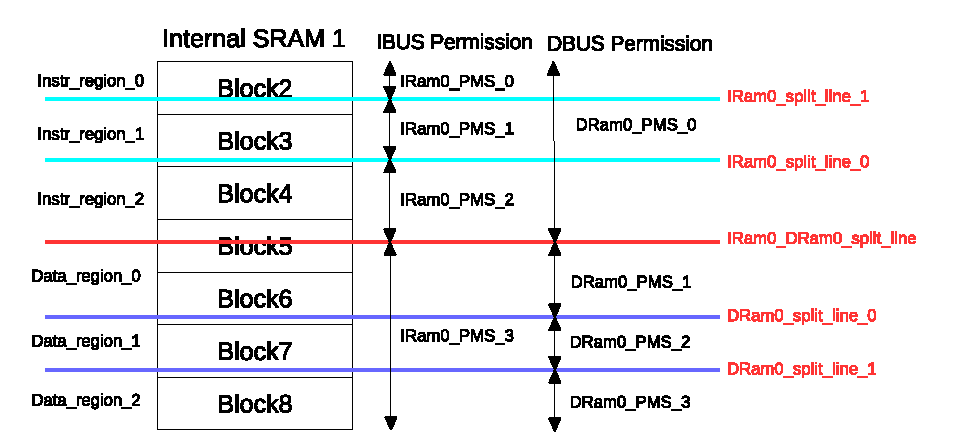
\includegraphics[width=0.7\textwidth]{./10-PERMCTRL/figures/pms_split_line.eps}
        \caption{Split Lines for Internal SRAM1}
        \label{fig:permctrl_region_split}
    \end{figure}

\begin{table}[H]
\caption{Internal SRAM1 Split Regions}
\label{tab:permctrl_region_split}
\centering
\begin{threeparttable}
\begin{tabular}{|L{3cm}|L{6cm}|L{6cm}|}
\hline
\rowcolor{lightgray}
\textbf{Internal Memory \tnote{A}}                     & \textbf{Instruction/Data Regions}                                & \textbf{Split Regions\tnote{B}}             \\ \hline
\multirow{6}{*}{SRAM1} & \multirow{3}{*}{Instruction Region} & Instr\_Region\_0 \\ \cline{3-3}
                       &                                     & Instr\_Region\_1 \\ \cline{3-3}
                       &                                     & Instr\_Region\_2 \\ \cline{2-3}
                       & \multirow{3}{*}{Data   Region}      & Data\_Region\_0  \\ \cline{3-3}
                       &                                     & Data\_Region\_1  \\ \cline{3-3}
                       &                                     & Data\_Region\_2  \\ \hline
\end{tabular}
    \begin{tablenotes}
        \item[A] See description below on how to configure the split lines.
        \item[B] Access to each split region can be configured independently. See details in Table \ref{tab:permctrl_sram1_inst_permsplit} and \ref{tab:permctrl_sram1_data_permsplit}.
    \end{tablenotes}
\end{threeparttable}
\end{table}

\subparagraph{Internal SRAM1 Split Regions}\label{sec:permctrl-split-line}

\chipname{} allows users to configure the split lines to their needs with registers below:
\begin{itemize}
    \item Split line to split the Instruction and Data regions (IRam0\_DRam0\_split\_line):
    \begin{itemize}
        \item \hyperref[regdesc:PMSCOREXIRAM0DRAM0DMASPLITLINECONSTRAIN1REG]{PMS\_CORE\_X\_IRAM0\_DRAM0\_DMA\_SPLIT\_LINE\_CONSTRAIN\_1\_REG}
    \end{itemize}
    \item The first split line to further split the Instruction Region (IRam0\_split\_line\_0):
    \begin{itemize}
        \item \hyperref[regdesc:PMSCOREXIRAM0DRAM0DMASPLITLINECONSTRAIN2REG]{PMS\_CORE\_X\_IRAM0\_DRAM0\_DMA\_SPLIT\_LINE\_CONSTRAIN\_2\_REG}
    \end{itemize}
    \item The second split line to further split the Instruction Region (IRam0\_split\_line\_1):
    \begin{itemize}
        \item \hyperref[regdesc:PMSCOREXIRAM0DRAM0DMASPLITLINECONSTRAIN3REG]{PMS\_CORE\_X\_IRAM0\_DRAM0\_DMA\_SPLIT\_LINE\_CONSTRAIN\_3\_REG}
    \end{itemize}
    \item The first split line to further split the data Region (DRam0\_split\_line\_0):
    \begin{itemize}
        \item \hyperref[regdesc:PMSCOREXIRAM0DRAM0DMASPLITLINECONSTRAIN4REG]{PMS\_CORE\_X\_IRAM0\_DRAM0\_DMA\_SPLIT\_LINE\_CONSTRAIN\_4\_REG}
    \end{itemize}
    \item The second split line to further split the data Region (DRam0\_split\_line\_1):
    \begin{itemize}
        \item \hyperref[regdesc:PMSCOREXIRAM0DRAM0DMASPLITLINECONSTRAIN5REG]{PMS\_CORE\_X\_IRAM0\_DRAM0\_DMA\_SPLIT\_LINE\_CONSTRAIN\_5\_REG}
    \end{itemize}
\end{itemize}

When configuring the split lines,
\begin{enumerate}
    \item First configure the block in which the spilt line is by:
    \begin{itemize}
        \item Configuring the Category\_\regindex{x} field for the block in which the split line is to 0x{}1 or 0x{}2 (no difference)
        \item Configuring the Category\_0 \verb+~+ Category\_\regindex{x-1} fields for all the preceding blocks to 0x{}0
        \item Configuring the Category\_\regindex{x+1} \verb+~+ Category\_6 fields for all blocks afterwards to 0x{}3
    \end{itemize}
        For example, assuming you want to configure the split line in Block5, then first configure the Category\_3 field for Block5 to 0x{}1 or 0x{}2; configure the Category\_0 \verb+~+ Category\_2 fields for Block2 \verb+~+ Block4 to 0x{}0; and configure the Category\_4 \verb+~+ Category\_6 fields for Block6 \verb+~+ Block8 to 0x{}3 (see illustration in Figure \ref{fig:PERMCTRL_category_config}). On the other hand, when reading 0x{}1 or 0x{}2 from Category\_3, then you know the split line is in Block5.
    \item Configure the position of the split line inside of the configured block by:
    \begin{itemize}
        \item Writing the [15:8] bits of the actual address at which you want to split the memory to the \hyperref[fielddesc:PMSCOREXIRAM0SRAMLINE0SPLITADDR]{SPLITADDR} field for the block in which the split line is.
        \item Note that the split address must be aligned to 256 bytes, meaning you can only write the integral multiples of 0x{}100 to the \hyperref[fielddesc:PMSCOREXIRAM0SRAMLINE0SPLITADDR]{SPLITADDR} field.
    \end{itemize}
        For example, if you want to split the instruction region at 0x{}3fc88000, then write the [15:8] bits of this address, which is 0b10000000, to \hyperref[fielddesc:PMSCOREXIRAM0SRAMLINE0SPLITADDR]{SPLITADDR}.
\end{enumerate}

\begin{figure}[!ht]
        \centering
        
\includegraphics[width=0.5\textwidth]{./10-PERMCTRL/figures/split_line_category.eps}
        \caption{An illustration of Configuring the Category fields}
        \label{fig:PERMCTRL_category_config}
\end{figure}

Note the following points when configuring the split lines:

 \begin{itemize}
     \item Position:
     \begin{itemize}
         \item The split line that splitting the Instruction Region and Data Region can be configured anywhere inside Internal SRAM1.
         \item The two split lines further splitting the Instruction Region into 3 split regions must stay inside the Instruction Region.
         \item The two split lines further splitting the Data Region into 3 split regions must stay inside the Data Region.
     \end{itemize}
     \item Spilt lines can overlap with each other. For example,
     \begin{itemize}
         \item When the two split lines inside the Data Region are not overlapping with each other, then the Data Region is split into 3 split regions
         \item When the two split lines inside the Data Region are overlapping with each other, then the Data Region is only split into 2 split regions
         \item When the two split lines inside the Data Region are not only overlapping with each other but also with the split line that splits the Data Region and the Instruction Region, then the Data Region is not split at all and only has one region.
     \end{itemize}
     \end{itemize}

\subparagraph{Access Configuration}

After configuring the split lines, users can then use the registers described in the Table \ref{tab:permctrl_sram1_inst_permsplit} and Table \ref{tab:permctrl_sram1_data_permsplit} below to configure the access of CPU's IBUS, DBUS and GDMA peripherals, from the Secure World and Non-secure World, to these split regions independently.

\begin{table}[H]
    \centering
    \caption{Access Configuration to the Instruction Region of Internal SRAM1}
    \label{tab:permctrl_sram1_inst_permsplit}

    \begin{threeparttable}
    \begin{tabular}{ |l|l|l|c|c|c|l| }
    \hline
    \rowcolor{lightgray}
        & & & \multicolumn{3}{c|}{\textbf{Instruction Region}} &  \\\cline{4-6}
    \rowcolor{lightgray}
    \multirow{-2}*{\textbf{Buses}}   & \multirow{-2}*{\textbf{From World}} & \multirow{-2}*{\textbf{Configuration Registers}} & \scriptsize{\textbf{instr\_region\_0}} & \scriptsize{\textbf{instr\_region\_1}} & \scriptsize{\textbf{instr\_region\_2}} & \multirow{-2}*{\textbf{Access}}   \\\hline
    \multirow{2}*{IBUS}             & Secure World        & \scriptsize{\hyperref[regdesc:PMSCOREXIRAM0PMSCONSTRAIN2REG]{PMS\_CORE\_X\_IRAM0\_PMS\_CONSTRAIN\_2\_REG}} & [2:0] & [5:3] & [8:6] & X/W/R \\\cline{2-7}
                                    & Non-secure World      & \scriptsize{\hyperref[regdesc:PMSCOREXIRAM0PMSCONSTRAIN1REG]{PMS\_Core\_X\_IRAM0\_PMS\_CONSTRAIN\_1\_REG}} & [2:0] & [5:3] & [8:6] & X/W/R \\\hline

     \multirow{2}*{DBUS}            & Secure World        &                                                                             & \multicolumn{3}{c|}{[1:0]\tnote{A}} & W/R \\ \cline{2-2} \cline{4-7}
                                    & Non-secure World      & \multirow{-2}*{\scriptsize{\hyperref[regdesc:PMSCOREXDRAM0PMSCONSTRAIN1REG]{PMS\_Core\_X\_DRAM0\_PMS\_CONSTRAIN\_1\_REG}}}      & \multicolumn{3}{c|}{[13:12]\tnote{A}}  & W/R \\\hline
    GDMA                        & \regindex{XX} Peripherals \tnote{C}             & \scriptsize{\hyperref[regdesc:PMSDMAAPBPERISPI2PMSCONSTRAIN1REG]{PMS\_DMA\_APBPERI\_\regindex{XX}\_PMS\_CONSTRAIN\_1\_REG}}  &   \multicolumn{3}{c|}{[1:0]\tnote{B}}   & W/R \\\hline

    \end{tabular}
        \begin{tablenotes}
            \item [A] Configure DBUS' access to the Instruction Region. However, it's recommended to configure these bits to 0.
            \item [B] Configure GDMA's access to the Instruction Region. However, it's recommended to configure these bits to 0.
            \item [C] \chipname{} has 9 peripherals, including SPI2, SPI3, UCHI0, I2S0, I2S1, AES, SHA, ADC, LCD\_CAM, USB, SDIO\_HOST, and RMT, which can access Internal SRAM1 via GDMA. Each peripherals can be configured with different access to the Internal SRAM1 independently.
        \end{tablenotes}
     \end{threeparttable}
    \end{table}

\begin{table}[H]
    \centering
    \caption{Access Configuration to the Data Region of Internal SRAM1}
    \label{tab:permctrl_sram1_data_permsplit}

    \begin{threeparttable}
    \begin{tabular}{ |l|L{2cm}|l|c|c|c|l| }
    \hline
    \rowcolor{lightgray}
        & & & \multicolumn{3}{c|}{\textbf{Data Region}} &  \\\cline{4-6}
    \rowcolor{lightgray}
    \multirow{-2}*{\textbf{Buses}}   & \multirow{-2}*{\textbf{From World}} & \multirow{-2}*{\textbf{Configuration Registers}} & \scriptsize{\textbf{data\_region\_0}} & \scriptsize{\textbf{data\_region\_1}} & \scriptsize{\textbf{data\_region\_2}} & \multirow{-2}*{\textbf{Access}}   \\\hline
     \multirow{2}*{IBUS}            & Secure World        &     \scriptsize{\hyperref[regdesc:PMSCOREXIRAM0PMSCONSTRAIN2REG]{PMS\_CORE\_X\_IRAM0\_PMS\_CONSTRAIN\_2\_REG}}                                                                                      & \multicolumn{3}{c|}{[11:9]\tnote{A}}  & X/W/R \\ \cline{2-7}
                                    & Non-secure World      & \scriptsize{\hyperref[regdesc:PMSCOREXIRAM0PMSCONSTRAIN1REG]{PMS\_CORE\_X\_IRAM0\_PMS\_CONSTRAIN\_1\_REG}}      & \multicolumn{3}{c|}{[11:9]\tnote{A}}  & X/W/R \\\hline
    \multirow{2}*{DBUS}             & Secure World       &                                                                                    & [3:2] & [5:4] & [7:6] & W/R \\\cline{2-2} \cline{4-7}
                                    & Non-secure World      & \multirow{-2}*{\scriptsize{\hyperref[regdesc:PMSCOREXDRAM0PMSCONSTRAIN1REG]{PMS\_Core\_X\_DRAM0\_PMS\_CONSTRAIN\_1\_REG}}} & [15:14] & [17:16] & [19:18] & W/R \\\hline
    GDMA \regindex{XX} \tnote{B}                    &  -            & \scriptsize{\hyperref[regdesc:PMSDMAAPBPERISPI2PMSCONSTRAIN1REG]{PMS\_DMA\_APBPERI\_\regindex{XX}\_PMS\_CONSTRAIN\_1\_REG}}  &  [3:2] & [5:4] & [7:6]    & W/R \\\hline

    \end{tabular}
        \begin{tablenotes}
            \item [A] Configure IBUS' access to the Data Region. However, it's recommended to configure these bits to 0.
            \item [B] \chipname{} has 9 peripherals, including SPI2, SPI3, UCHI0, I2S0, I2S1, AES, SHA, ADC, LCD\_CAM, USB, SDIO\_HOST, and RMT, which can access Internal SRAM1 via GDMA. Each peripherals can be configured with different access to the Internal SRAM1 independently.
            \end{tablenotes}
     \end{threeparttable}
\end{table}

For details on how to configure the split lines, see Section \ref{sec:permctrl-split-line}.

\subparagraph{Trace Memory} \label{sec:permctrl_trace}
\chipname{} has a low-power Xtensa® dual-core 32-bit LX7 microprocessor, which integrates a TRAX (Real-time Trace) module for easier debugging. For the TRAX module to work, users need to allocate 16 KB from the Internal SRAM1 as Trace memory. Note that, the Trace memories for CPU0 and CPU1 can be configured independently.

Users can allocate 16 KB from Internal SRAM1 as Trace memory by configuring the  \hyperref[regdesc:PMSINTERNALSRAMUSAGE2REG]{PMS\_INTERNAL\_SRAM\_USAGE\_2\_REG} register.

Detailed steps are provided below:

\begin{enumerate}
    \item First choose a block from Block2 \verb+~+ Block8 by writing 1 to the respective bit in the \\ \hyperref[fielddesc:PMSINTERNALSRAMCORE0TRACEUSAGE]{PMS\_INTERNAL\_SRAM\_CORE\regindex{m}\_TRACE\_USAGE} field
    \begin{itemize}
        \item Block2: 0b00000001
        \item Block3: 0b00000010
        \item Block4: 0b00000100
        \item Block5: 0b00001000
        \item Block6: 0b00010000
        \item Block7: 0b00100000
        \item Block8: 0b01000000
    \end{itemize}
    \item Then choose 16 KB from this block as the Trace memory by configuring the \\ \hyperref[fielddesc:PMSINTERNALSRAMCORE0TRACEALLOC]{PMS\_INTERNAL\_SRAM\_CORE\regindex{m}\_TRACE\_ALLOC} field
    \begin{itemize}
        \item 2'b00: the first 16 KB
        \item 2'b01: the second 16 KB
        \item 2'b10: the third 16 KB
        \item 2'b11: the fourth 16 KB
    \end{itemize}
    Note that Block2 is only 32 KB, so you can only configure this field to 2'b00 or 2'b0 when Block2 is selected in the first step.
\end{enumerate}

For example, if you want to choose the first 16 KB of Internal SRAM1 Block3's as CPU0's trace memory, then you need to:
\begin{itemize}
    \item Write 0b0000010 to the \hyperref[fielddesc:PMSINTERNALSRAMCORE0TRACEUSAGE]{PMS\_INTERNAL\_SRAM\_CORE0\_TRACE\_USAGE} field to select Block3
    \item Write 2'b00 to the \hyperref[fielddesc:PMSINTERNALSRAMCORE0TRACEALLOC]{PMS\_INTERNAL\_SRAM\_CORE0\_TRACE\_ALLOC} field to select the first 16 KB.
\end{itemize}

\subsubsection{Internal SRAM2  Access Configuration}\label{sec:permctrl_sram2}

\chipname{}'s Internal SRAM2 includes Block9 and Block10 (see details in Table \ref{tab:permctrl-SRAM_block_address}), which can be allocated to either CPU/GDMA or DCACHE. Note that once configured, the configuration applies to both CPU0 and CPU1.

\chipname{} uses registers described in Table \ref{tab:permctrl-sram2_accessconfig} to configure the Internal SRAM2 for CPU/GDMA or DCACHE.

\begin{table}[H]
    \centering
    \caption{Internal SRAM2 Usage Configuration}
    \label{tab:permctrl-sram2_accessconfig}
    \begin{threeparttable}
    \begin{tabular}{|l|l|c|}
    \hline
    \rowcolor{lightgray}
                          &\textbf{Block}  & \textbf{\hyperref[regdesc:PMSINTERNALSRAMUSAGE1REG]{PMS\_INTERNAL\_SRAM\_USAGE\_1\_REG}\tnote{A}}\\\hline
    \multirow{2}{*}{SRAM} & Block9\tnote{B}        & [3] \\\cline{2-3}
                          & Block10        & [2] \\\hline
    \end{tabular}
        \begin{tablenotes}
        \item[A] Set this bit to allocate a certain block to CPU/GDMA. Clear this bit to allocate a certain block to DCACHE.
        \item[B] For example, setting this bit indicates Block9 is allocated to CPU/GDMA.
        \end{tablenotes}
    \end{threeparttable}
\end{table}

When a certain block is allocated to CPU/GDMA, \chipname{} uses the registers listed in Table \ref{tab:permctrl-SRAM2_block_address} to configure the write (W) and read (R) accesses of CPU's DBUS, from the Secure World and Non-secure World, to this block:

\begin{table}[H]
    \centering
    \caption{Access Configuration to Internal SRAM2}
    \label{tab:permctrl-SRAM2_block_address}
    \begin{threeparttable}
    \begin{tabular}{ |l|l|l|l|l|l|}
    \hline
        \rowcolor{lightgray}
        & & & \multicolumn{2}{c|}{\textbf{SRAM2}} &  \\\cline{4-5}
        \rowcolor{lightgray}
        \multirow{-2}*{\textbf{Bus \tnote{A}}}   & \multirow{-2}*{\textbf{From World}} & \multirow{-2}*{\textbf{Configuration Registers}} & \textbf{Block9} & \textbf{Block10} & \multirow{-2}*{\textbf{Access}\tnote{B}} \\\hline
        % table contents
        \multirow{2}*{DBUS} & Secure World   & \hyperref[regdesc:PMSCOREXDRAM0PMSCONSTRAIN1REG]{PMS\_CORE\_X\_DRAM0\_PMS\_CONSTRAIN\_1\_REG}& [9:8]\tnote{C} & [11:10] & W/R \\\cline{2-6}
                            & Non-secure World & \hyperref[regdesc:PMSCOREXDRAM0PMSCONSTRAIN1REG]{PMS\_CORE\_X\_DRAM0\_PMS\_CONSTRAIN\_1\_REG} & [21:20] & [23:22] & W/R \\\hline
        GDMA                    & \regindex{XX} Peripherals\tnote{B}              & \hyperref[regdesc:PMSDMAAPBPERISPI2PMSCONSTRAIN1REG]{PMS\_DMA\_APBPERI\_\regindex{XX}\_PMS\_CONSTRAIN\_1\_REG}  &  [9:8] & [11:10]    & W/R \\\hline
        \end{tabular}
        \begin{tablenotes}
            \item[A] To access the Internal SRAM2, the CPU/GDMA must be configured with both the \hyperref[tab:permctrl-sram2_accessconfig]{usage} permission and respective access permission.
            \item[B] 1: with access; 0: without access
            \item[C] For example, configuring this field to 0b10 indicates CPU's DBUS is granted with write access but not read access from the Secure World to the Block9 of Internal SRAM2.
        \end{tablenotes}
        \end{threeparttable}
    \end{table}

\subsection{RTC FAST Memory}

\subsubsection{Address}

\chipname{}'s RTC FAST Memory is 8 KB. See the address of RTC FAST Memory below:

\begin{longtable}[c]{ |l|l|l| }
\caption{RTC FAST Memory Address}
\label{tab:fast-memory-address}
\\\hline
\rowcolor{lightgray}
    \textbf{Memory} &  \textbf{Starting Address}  &  \textbf{Ending Address}\\
    \hline
    RTC FAST Memory           & 0x{}600F\_E000 &  0x{}600F\_FFFF   \\
    \hline
\end{longtable}

\subsubsection{Access Configuration}

\chipname{}'s RTC FAST Memory can be further split into 2 regions. Each split region can be configured independently with different access by configuring respective registers (\hyperref[regdesc:PMSCORE0PIFPMSCONSTRAIN1REG]{PMS\_CORE\_\regindex{m}\_PIF\_PMS\_CONSTRAN\_\regindex{n}\_REG}).

Note that split regions can be configured independently for CPU0 and CPU1 and for the Secure World and Non-secure World.

The Register for configuring the split line is described below:
\begin{table}[H]
    \centering
    \caption{Split RTC FAST Memory into the Higher Region and the Lower Region}
    \label{tab:rtc_fast_mem_split}
    \begin{threeparttable}
    \begin{tabular}{|l|l|l|l|} \hline
    \rowcolor{lightgray}
     & & \multicolumn{2}{c|}{\textbf{Configuration Register}\tnote{1}} \\\cline{3-4}
    \rowcolor{lightgray}
    \multirow{-2}*{\textbf{Memory}} & \multirow{-2}*{\textbf{Split Regions}}  & \textbf{Secure World} & \textbf{Non-secure World} \\\hline
    \multirow{2}*{RTC FAST Memory} & Higher Region &                   &       \\\cline{2-2}
    & Lower Region & \multirow{-2}*{\hyperref[regdesc:PMSCORE0PIFPMSCONSTRAIN9REG]{PIF\_PMS\_CONSTRAN\_9\_REG} [10:0]}  & \multirow{-2}*{\hyperref[regdesc:PMSCORE0PIFPMSCONSTRAIN9REG]{PIF\_PMS\_CONSTRAN\_9\_REG} [21:11]} \\\hline
    \end{tabular}
        \begin{tablenotes}
        \item[1] The offset from the RTC FAST Memory base address should be used when configuring the split address. For example, if you want to split the RTC FAST Memory at 0x{}600F\_F000, then write 0x{}1000 to this register.
        \end{tablenotes}
    \end{threeparttable}
\end{table}

Access configuration for the higher and lower regions of the RTC FAST Memory is described below:
\begin{table}[H]
    \centering
    \caption{Access Configuration to the RTC FAST Memory}
    \label{tab:rtc_fast_mem_split_access}
    \begin{threeparttable}
    \begin{tabular}{|l|c|l|l|l|} \hline
    \rowcolor{lightgray}
     &\textbf{RTC}  & \multicolumn{2}{c|}{\textbf{Configuration Registers}}& \\\cline{3-4}
    \rowcolor{lightgray}
    \multirow{-2}*{\textbf{Bus}}   & \textbf{FAST Memory} & \textbf{Secure World} & \textbf{Non-secure World} & \multirow{-2}*{\textbf{Access}\tnote{A}} \\\hline
     Peri Bus    & Higher Region                       &   \hyperref[regdesc:PMSCORE0PIFPMSCONSTRAIN10REG]{PIF\_PMS\_CONSTRAN\_10\_REG} [5:3] \tnote{B}               &    \hyperref[regdesc:PMSCORE0PIFPMSCONSTRAIN10REG]{PIF\_PMS\_CONSTRAN\_10\_REG} [11:9]  & \\\cline{2-4}
      (PIF) & Lower Region & \hyperref[regdesc:PMSCORE0PIFPMSCONSTRAIN10REG]{PIF\_PMS\_CONSTRAN\_10\_REG} [2:0] & \hyperref[regdesc:PMSCORE0PIFPMSCONSTRAIN10REG]{PIF\_PMS\_CONSTRAN\_10\_REG} [8:6]  & \multirow{-2}*{X/W/R}  \\\hline
    \end{tabular}
        \begin{tablenotes}
        \item[A] 1: with access; 0: without access
        \item[B] For example, configuring this field to 0b101 indicates CPU's peripheral (PIF) bus is granted with the instruction execution and read accesses but not the read access from the Secure WORLD to the higher region of RTC FAST Memory.
        \end{tablenotes}
    \end{threeparttable}
\end{table}

\subsection{RTC SLOW Memory}

\subsubsection{Address}

\chipname{}'s RTC SLOW Memory is 8 KB. This memory can be accessed using two addresses, i.e, RTCSlow\_0 and RTCSlow\_1. See details in Table \ref{tab:slow-memory-address} below:

\begin{longtable}[c]{ |c|l|l| }
\caption{RTC SLOW Memory Address}
\label{tab:slow-memory-address}
\\\hline
\rowcolor{lightgray}
    \textbf{RTC SLOW Memory} &  \textbf{Starting Address}  &  \textbf{Ending Address}\\
    \hline
    RTCSlow\_0           & 0x{}5000\_0000 &  0x{}5000\_1FFF   \\
    \hline
    RTCSlow\_1           & 0x{}6002\_1000 &  0x{}6002\_2FFF   \\
    \hline
\end{longtable}


\subsubsection{Access Configuration}

Both \chipname{}'s RTCSlow\_0 and RTCSlow\_1 can be further split into 2 regions. Each split region can be configured independently with different access by configuring respective registers (\hyperref[regdesc:PMSCORE0PIFPMSCONSTRAIN1REG]{PMS\_CORE\_\regindex{m}\_PIF\_PMS\_CONSTRAN\_\regindex{n}\_REG}).

Note that split regions can be configured independently for CPU0 and CPU1 and for the Secure World and Non-secure World.

The registers for splitting RTC SLOW Memory into 4 split regions are described below:
\begin{table}[H]
    \centering
    \caption{Split RTCSlow\_0 and RTCSlow\_1 into Split Regions}
    \label{tab:rtc_slow_mem_split}
    \begin{threeparttable}
    \begin{tabular}{|l|l|l|l|} \hline
    \rowcolor{lightgray}
    & & \multicolumn{2}{c|}{\textbf{Configuration Registers}\tnote{1}} \\\cline{3-4}
    \rowcolor{lightgray}
    \multirow{-2}*{\textbf{Memory}} & \multirow{-2}*{\textbf{Split Regions}}  & \textbf{Secure World} & \textbf{Non-secure World} \\\hline
     & Higher Region &                   &       \\\cline{2-2}
    \multirow{-2}*{RTCSlow\_0} & Lower Region & \multirow{-2}*{\hyperref[regdesc:PMSCORE0PIFPMSCONSTRAIN11REG]{PIF\_PMS\_CONSTRAN\_11\_REG} [10:0]}  & \multirow{-2}*{\hyperref[regdesc:PMSCORE0PIFPMSCONSTRAIN9REG]{PIF\_PMS\_CONSTRAN\_9\_REG} [21:11]} \\\hline
     & Higher Region &                   &       \\\cline{2-2}
    \multirow{-2}*{RTCSlow\_1} & Lower Region & \multirow{-2}*{\hyperref[regdesc:PMSCORE0PIFPMSCONSTRAIN13REG]{PIF\_PMS\_CONSTRAN\_13\_REG} [10:0]}  & \multirow{-2}*{\hyperref[regdesc:PMSCORE0PIFPMSCONSTRAIN13REG]{PIF\_PMS\_CONSTRAN\_13\_REG} [21:11]} \\\hline
    \end{tabular}
        \begin{tablenotes}
        \item[1] The offset from the RTC SLOW Memory base address should be used when configuring the split address. For example, if you want to split the RTC SLOW Memory at 0x{}6002\_2000, then write 0x{}1000 to this register.
        \end{tablenotes}
    \end{threeparttable}
\end{table}

Access configuration to the split regions of RTC SLOW Memory is described below:
\begin{table}[H]
    \centering
    \caption{Access Configuration to the RTC SLOW Memory}
    \label{tab:rtc_slow1_mem_pms_access}
    \begin{threeparttable}
    \begin{tabular}{ | l | l | c | l | l | l|}
    \hline
        \rowcolor{lightgray}
        & & \textbf{Split} & \multicolumn{2}{c|}{\textbf{Configuration Registers}} &  \\\cline{4-5}
        \rowcolor{lightgray}
        \multirow{-2}*{\textbf{Bus}}  & \multirow{-2}*{\textbf{Mem}} &  \textbf{Regions} & \textbf{Secure World} & \textbf{Non-secure World} & \multirow{-2}*{\textbf{Access}} \\\hline

         & RTC & Higher\tnote{A} & \hyperref[regdesc:PMSCORE0PIFPMSCONSTRAIN12REG]{PIF\_PMS\_CONSTRAN\_12\_REG} [5:3]\tnote{C} & \hyperref[regdesc:PMSCORE0PIFPMSCONSTRAIN12REG]{PIF\_PMS\_CONSTRAN\_12\_REG} [11:9] & \\\cline{3-5}
        \multirow{-2}*{Peri}  & Slow\_0 & Lower \tnote{B}& \hyperref[regdesc:PMSCORE0PIFPMSCONSTRAIN12REG]{PIF\_PMS\_CONSTRAN\_12\_REG} [2:0] & \hyperref[regdesc:PMSCORE0PIFPMSCONSTRAIN12REG]{PIF\_PMS\_CONSTRAN\_12\_REG} [8:6] & \\\cline{2-5}
        Bus & RTC & Higher\tnote{A} & \hyperref[regdesc:PMSCORE0PIFPMSCONSTRAIN14REG]{PIF\_PMS\_CONSTRAN\_14\_REG} [5:3] & \hyperref[regdesc:PMSCORE0PIFPMSCONSTRAIN14REG]{PIF\_PMS\_CONSTRAN\_14\_REG} [11:9] & \\\cline{3-5}
        (PIF)  & Slow\_1 & Lower\tnote{B} & \hyperref[regdesc:PMSCORE0PIFPMSCONSTRAIN14REG]{PIF\_PMS\_CONSTRAN\_14\_REG} [2:0] & \hyperref[regdesc:PMSCORE0PIFPMSCONSTRAIN14REG]{PIF\_PMS\_CONSTRAN\_14\_REG} [8:6] & \multirow{-4}*{X/W/R} \\\hline

        \end{tabular}

        \begin{tablenotes}
        \item[A] Higher is short for Higher Region.
        \item[B] Lower is short for Lower Region.
        \item[C] For example, configuring this field to 0b100 indicates CPU's peripheral (PIF) bus is granted with the instruction execution access but not the write or read accesses from the Secure WORLD to the higher region of RTCSLOW\_0.
        \end{tablenotes}
    \end{threeparttable}
\end{table}


\section{Peripherals}
\subsection{Access Configuration}\label{sec:permctrl-peri-address}

\chipname{}'s CPU can be configured with different read (R) and write (W) accesses to most of its modules and peripherals independently, from the Secure World and the Non-secure World, by configuring respective registers (\hyperref[regdesc:PMSCORE0PIFPMSCONSTRAIN1REG]{PMS\_CORE\_\regindex{m}\_PIF\_PMS\_CONSTRAN\_\regindex{n}\_REG}).

Note that permission to modules and peripherals can be configured independently for CPU0 and CPU1 and for the Secure World and Non-secure World.

Notes on \hyperref[regdesc:PMSCORE0PIFPMSCONSTRAIN1REG]{PMS\_CORE\_\regindex{m}\_PIF\_PMS\_CONSTRAN\_\regindex{n}\_REG}:
\begin{itemize}
    \item \regindex{m} can be 0 or 1 for CPU0 and CPU1 respectively.
    \item \regindex{n} can be 1\verb+~+8, in which 1\verb+~+4 are for Secure World and 5\verb+~+8 are for Non-secure World.
\end{itemize}

For example, users can configure  \hyperref[regdesc:PMSCORE0PIFPMSCONSTRAIN1REG]{PMS\_CORE\_0\_PIF\_PMS\_CONSTRAIN\_1\_REG [1:0]} to 0x{}2, meaning CPU0 is granted with read access but not write access from the Secure World to UART0. In this case, CPU0 won't be able to modify the UART0's internal registers when in Secure World.
\begin{ThreePartTable}

\begin{TableNotes}
\item[1]: Accelerators: AES, SHA, RSA, Digital Signatures, HMAC
\item[2]: This is shared by more than one peripherals.
\item[3]: Access: R/W
\end{TableNotes}

\begin{longtable}[c]{ |l|l|l|l| }
    \caption{Access Configuration of the Peripherals}
    \label{tab:permctrl-peripheral-controlling-bit}
    \\\hline\rowcolor{lightgray}
    \textbf{Peripherals}    & \textbf{Secure World} & \textbf{Non-secure World} & \textbf{Bit}\tnote{3}\\\hline
    \endfirsthead
    \multicolumn{3}{c}{\bfseries \tablename\ \thetable{} -- cont'd from previous page}\\\hline
    \rowcolor{lightgray}
    \textbf{Peripherals}    & \textbf{Secure World} & \textbf{Non-secure World} & \textbf{Bit}\tnote{3}\\\hline
    \endhead
    \multicolumn{3}{r}{\textbf{Cont'd on next page}} \\
    \endfoot
    \insertTableNotes
    \endlastfoot
    GDMA  & PIF\_PMS\_CONSTRAN\_4\_REG & PIF\_PMS\_CONSTRAN\_8\_REG & [7:6] \\\hline
    eFuse Controller \& PMU\tnote{2} & PIF\_PMS\_CONSTRAN\_1\_REG & PIF\_PMS\_CONSTRAN\_5\_REG & [15:14] \\\hline
    IO\_MUX & PIF\_PMS\_CONSTRAN\_1\_REG & PIF\_PMS\_CONSTRAN\_5\_REG & [17:16] \\\hline
    GPIO & PIF\_PMS\_CONSTRAN\_1\_REG & PIF\_PMS\_CONSTRAN\_5\_REG & [7:6] \\\hline
    Interrupt Matrix & PIF\_PMS\_CONSTRAN\_4\_REG & PIF\_PMS\_CONSTRAN\_8\_REG & [21:20] \\\hline
    System Timer & PIF\_PMS\_CONSTRAN\_2\_REG & PIF\_PMS\_CONSTRAN\_6\_REG & [31:30] \\\hline
    Timer Group 0 & PIF\_PMS\_CONSTRAN\_2\_REG & PIF\_PMS\_CONSTRAN\_6\_REG & [27:26] \\\hline
    Timer Group 1 & PIF\_PMS\_CONSTRAN\_2\_REG & PIF\_PMS\_CONSTRAN\_6\_REG & [29:28] \\\hline
    World Controller & PIF\_PMS\_CONSTRAN\_4\_REG & PIF\_PMS\_CONSTRAN\_8\_REG & [31:30] \\\hline
    System Registers & PIF\_PMS\_CONSTRAN\_4\_REG & PIF\_PMS\_CONSTRAN\_8\_REG & [17:16] \\\hline
    Sensitive Registers & PIF\_PMS\_CONSTRAN\_4\_REG & PIF\_PMS\_CONSTRAN\_8\_REG & [19:18] \\\hline
    Accelerators\tnote{1} & PIF\_PMS\_CONSTRAN\_4\_REG & PIF\_PMS\_CONSTRAN\_8\_REG & [5:4] \\\hline
    CACHE \& XTS\_AES\tnote{2} & PIF\_PMS\_CONSTRAN\_4\_REG & PIF\_PMS\_CONSTRAN\_8\_REG & [25:25] \\\hline
    UART 0 & PIF\_PMS\_CONSTRAN\_1\_REG & PIF\_PMS\_CONSTRAN\_5\_REG & [1:0] \\\hline
    UART 1 & PIF\_PMS\_CONSTRAN\_1\_REG & PIF\_PMS\_CONSTRAN\_5\_REG & [31:30] \\\hline
    UART 2 & PIF\_PMS\_CONSTRAN\_3\_REG & PIF\_PMS\_CONSTRAN\_7\_REG & [17:16] \\\hline
    SPI 0 & PIF\_PMS\_CONSTRAN\_1\_REG & PIF\_PMS\_CONSTRAN\_5\_REG & [5:4] \\\hline
    SPI 1 & PIF\_PMS\_CONSTRAN\_1\_REG & PIF\_PMS\_CONSTRAN\_5\_REG & [3:2] \\\hline
    SPI 2 & PIF\_PMS\_CONSTRAN\_3\_REG & PIF\_PMS\_CONSTRAN\_7\_REG & [1:0] \\\hline
    SPI 3 & PIF\_PMS\_CONSTRAN\_3\_REG & PIF\_PMS\_CONSTRAN\_7\_REG & [3:2] \\\hline
    I2C 0 & PIF\_PMS\_CONSTRAN\_2\_REG & PIF\_PMS\_CONSTRAN\_6\_REG & [5:4] \\\hline
    I2C 1 & PIF\_PMS\_CONSTRAN\_3\_REG & PIF\_PMS\_CONSTRAN\_7\_REG & [7:6] \\\hline
    I2S 0 & PIF\_PMS\_CONSTRAN\_1\_REG & PIF\_PMS\_CONSTRAN\_5\_REG & [29:28] \\\hline
    I2S 1 & PIF\_PMS\_CONSTRAN\_3\_REG & PIF\_PMS\_CONSTRAN\_7\_REG & [15:14] \\\hline
    Pulse Count Controller & PIF\_PMS\_CONSTRAN\_2\_REG & PIF\_PMS\_CONSTRAN\_6\_REG & [13:12] \\\hline
    USB Serial/JTAG Controller & PIF\_PMS\_CONSTRAN\_4\_REG & PIF\_PMS\_CONSTRAN\_8\_REG & [1:0] \\\hline
    USB OTG Core & PIF\_PMS\_CONSTRAN\_4\_REG & PIF\_PMS\_CONSTRAN\_8\_REG & [15:14] \\\hline
    USB OTG External & PIF\_PMS\_CONSTRAN\_4\_REG & PIF\_PMS\_CONSTRAN\_8\_REG & [3:2] \\\hline
    Two-wire Automotive Interface & PIF\_PMS\_CONSTRAN\_3\_REG & PIF\_PMS\_CONSTRAN\_7\_REG & [11:10] \\\hline
    UHCI 0  & PIF\_PMS\_CONSTRAN\_2\_REG & PIF\_PMS\_CONSTRAN\_6\_REG & [7:6] \\\hline
    SD/MMC Host Controller & PIF\_PMS\_CONSTRAN\_3\_REG & PIF\_PMS\_CONSTRAN\_7\_REG & [9:8] \\\hline
    LED PWM Controller  & PIF\_PMS\_CONSTRAN\_2\_REG & PIF\_PMS\_CONSTRAN\_6\_REG & [17:16] \\\hline
    Motor Control PWM 0 & PIF\_PMS\_CONSTRAN\_2\_REG & PIF\_PMS\_CONSTRAN\_6\_REG & [25:24] \\\hline
    Motor Control PWM 1 & PIF\_PMS\_CONSTRAN\_3\_REG & PIF\_PMS\_CONSTRAN\_7\_REG & [13:12] \\\hline
    Remote Control Peripheral  & PIF\_PMS\_CONSTRAN\_2\_REG & PIF\_PMS\_CONSTRAN\_6\_REG & [11:10] \\\hline
    Camera-LCD Controller & PIF\_PMS\_CONSTRAN\_4\_REG & PIF\_PMS\_CONSTRAN\_8\_REG & [11:10] \\\hline
    APB Controller & PIF\_PMS\_CONSTRAN\_3\_REG & PIF\_PMS\_CONSTRAN\_7\_REG & [5:4] \\\hline
    ADC Controller & PIF\_PMS\_CONSTRAN\_4\_REG & PIF\_PMS\_CONSTRAN\_8\_REG & [9:8] \\\hline
\end{longtable}
\end{ThreePartTable}


\subsection{Split Peripheral Regions into Split Regions}

Each of \chipname{}'s peripheral region can be further split into 11 regions (from Peri Region0 \verb+~+ Peri Region10) for more flexible permission control.

For example, the registers for \chipname{}'s GDMA controller are allocated as:
\begin{itemize}
    \item 5 sets of registers for 5 of each RX channel
    \item 5 sets of registers for 5 of each TX channel
    \item 1 set of registers for configuration
\end{itemize}

As seen above, GDMA's peripheral region is divided into 11 split regions (implemented in hardware), which can be configured with different permission independently, thus achieving independent permission control to each GDMA channel.

Users can configure CPU's read (R) and write (W) accesses to a specific split region (Peri Region\regindex{n}) from the Secure World and the Non-secure World by configuring \hyperref[regdesc:PMSCORE0REGIONPMSCONSTRAIN1REG]{PMS\_CORE\_\regindex{m}\_Region\_PMS\_CONSTRAN\_\regindex{n}\_REG}. Note that permission can be configured independently for CPU0 and CPU1.

Notes on \hyperref[regdesc:PMSCORE0REGIONPMSCONSTRAIN1REG]{PMS\_CORE\_\regindex{m}\_Region\_PMS\_CONSTRAN\_\regindex{n}\_REG}:
\begin{itemize}
    \item \regindex{m} can be 0 or 1 for CPU0 and CPU1 respectively.
    \item \regindex{n} can be 1\verb+~+14, in which    \begin{itemize}
        \item \hyperref[regdesc:PMSCORE0REGIONPMSCONSTRAIN1REG]{Region\_PMS\_CONSTRAN\_1\_REG} is for configuring CPU's permission from the Secure World.
        \item \hyperref[regdesc:PMSCORE0REGIONPMSCONSTRAIN2REG]{Region\_PMS\_CONSTRAN\_2\_REG} is for configuring CPU's permission from the Non-secure World.
        \item \hyperref[regdesc:PMSCORE0REGIONPMSCONSTRAIN3REG]{Region\_PMS\_CONSTRAN\_\regindex{n}\_REG} (\regindex{n} = 3\verb+~+14) are used to configuring the starting addresses for each Peri Regions. Note the starting address of each Peri Region is also the ending address of the previous Peri Region.
    \end{itemize}
\end{itemize}


\begin{table}[H]
    \centering
    \caption{Access Configuration of Peri Regions}
    \label{tab:peri_mem_pms}
    \begin{tabular}{ | l | l | l | l |}
    \hline
        \rowcolor{lightgray}
         & & \multicolumn{2}{c|}{\textbf{Access Configuration}} \\\cline{3-4}
        \rowcolor{lightgray}
        \multirow{-2}*{\textbf{Peri Regions}} & \multirow{-2}*{\textbf{Starting Address Configuration}} & \textbf{Secure World} & \textbf{NOn-secure World}\\\hline
        Peri Region0 & \scriptsize{\hyperref[regdesc:PMSCORE0REGIONPMSCONSTRAIN3REG]{Region\_PMS\_CONSTRAN\_3\_REG}} & \scriptsize{\hyperref[regdesc:PMSCORE0REGIONPMSCONSTRAIN1REG]{\hyperref[regdesc:PMSCORE0REGIONPMSCONSTRAIN1REG]{Region\_PMS\_CONSTRAN\_1\_REG}} [1:0]} & \scriptsize{\hyperref[regdesc:PMSCORE0REGIONPMSCONSTRAIN1REG]{Region\_PMS\_CONSTRAN\_2\_REG} [1:0]}\\\hline
        Peri Region1 & \scriptsize{\hyperref[regdesc:PMSCORE0REGIONPMSCONSTRAIN3REG]{Region\_PMS\_CONSTRAN\_4\_REG}} & \scriptsize{\hyperref[regdesc:PMSCORE0REGIONPMSCONSTRAIN1REG]{Region\_PMS\_CONSTRAN\_1\_REG} [3:2]} & \scriptsize{\hyperref[regdesc:PMSCORE0REGIONPMSCONSTRAIN1REG]{Region\_PMS\_CONSTRAN\_2\_REG} [3:2]}\\\hline
        Peri Region2 & \scriptsize{\hyperref[regdesc:PMSCORE0REGIONPMSCONSTRAIN3REG]{Region\_PMS\_CONSTRAN\_5\_REG}} & \scriptsize{\hyperref[regdesc:PMSCORE0REGIONPMSCONSTRAIN1REG]{Region\_PMS\_CONSTRAN\_1\_REG} [5:4]} & \scriptsize{\hyperref[regdesc:PMSCORE0REGIONPMSCONSTRAIN1REG]{Region\_PMS\_CONSTRAN\_2\_REG} [5:4]}\\\hline
        Peri Region3 & \scriptsize{\hyperref[regdesc:PMSCORE0REGIONPMSCONSTRAIN3REG]{Region\_PMS\_CONSTRAN\_6\_REG}} & \scriptsize{\hyperref[regdesc:PMSCORE0REGIONPMSCONSTRAIN1REG]{Region\_PMS\_CONSTRAN\_1\_REG} [7:6]} & \scriptsize{\hyperref[regdesc:PMSCORE0REGIONPMSCONSTRAIN1REG]{Region\_PMS\_CONSTRAN\_2\_REG} [7:6]}\\\hline
        Peri Region4 & \scriptsize{\hyperref[regdesc:PMSCORE0REGIONPMSCONSTRAIN3REG]{Region\_PMS\_CONSTRAN\_7\_REG}} & \scriptsize{\hyperref[regdesc:PMSCORE0REGIONPMSCONSTRAIN1REG]{Region\_PMS\_CONSTRAN\_1\_REG} [9:8]} & \scriptsize{\hyperref[regdesc:PMSCORE0REGIONPMSCONSTRAIN1REG]{Region\_PMS\_CONSTRAN\_2\_REG} [9:8]}\\\hline
        Peri Region5 & \scriptsize{\hyperref[regdesc:PMSCORE0REGIONPMSCONSTRAIN3REG]{Region\_PMS\_CONSTRAN\_8\_REG}} & \scriptsize{\hyperref[regdesc:PMSCORE0REGIONPMSCONSTRAIN1REG]{Region\_PMS\_CONSTRAN\_1\_REG} [11:10]} & \scriptsize{\hyperref[regdesc:PMSCORE0REGIONPMSCONSTRAIN1REG]{Region\_PMS\_CONSTRAN\_2\_REG} [11:10]}\\\hline
        Peri Region6 & \scriptsize{\hyperref[regdesc:PMSCORE0REGIONPMSCONSTRAIN3REG]{Region\_PMS\_CONSTRAN\_9\_REG}} & \scriptsize{\hyperref[regdesc:PMSCORE0REGIONPMSCONSTRAIN1REG]{Region\_PMS\_CONSTRAN\_1\_REG} [13:12]} & \scriptsize{\hyperref[regdesc:PMSCORE0REGIONPMSCONSTRAIN1REG]{Region\_PMS\_CONSTRAN\_2\_REG} [13:12]}\\\hline
        Peri Region7 & \scriptsize{\hyperref[regdesc:PMSCORE0REGIONPMSCONSTRAIN3REG]{Region\_PMS\_CONSTRAN\_10\_REG}} & \scriptsize{\hyperref[regdesc:PMSCORE0REGIONPMSCONSTRAIN1REG]{Region\_PMS\_CONSTRAN\_1\_REG} [15:14]} & \scriptsize{\hyperref[regdesc:PMSCORE0REGIONPMSCONSTRAIN1REG]{Region\_PMS\_CONSTRAN\_2\_REG} [15:14]}\\\hline
        Peri Region8 & \scriptsize{\hyperref[regdesc:PMSCORE0REGIONPMSCONSTRAIN3REG]{Region\_PMS\_CONSTRAN\_11\_REG}} & \scriptsize{\hyperref[regdesc:PMSCORE0REGIONPMSCONSTRAIN1REG]{Region\_PMS\_CONSTRAN\_1\_REG} [17:16]} & \scriptsize{\hyperref[regdesc:PMSCORE0REGIONPMSCONSTRAIN1REG]{Region\_PMS\_CONSTRAN\_2\_REG} [17:16]}\\\hline
        Peri Region9 & \scriptsize{\hyperref[regdesc:PMSCORE0REGIONPMSCONSTRAIN3REG]{Region\_PMS\_CONSTRAN\_12\_REG}} & \scriptsize{\hyperref[regdesc:PMSCORE0REGIONPMSCONSTRAIN1REG]{Region\_PMS\_CONSTRAN\_1\_REG} [19:18]} & \scriptsize{\hyperref[regdesc:PMSCORE0REGIONPMSCONSTRAIN1REG]{Region\_PMS\_CONSTRAN\_2\_REG} [19:18]}\\\hline
        Peri Region10 & \scriptsize{\hyperref[regdesc:PMSCORE0REGIONPMSCONSTRAIN3REG]{Region\_PMS\_CONSTRAN\_13\_REG}} & \scriptsize{\hyperref[regdesc:PMSCORE0REGIONPMSCONSTRAIN1REG]{Region\_PMS\_CONSTRAN\_1\_REG} [21:20]} & \scriptsize{\hyperref[regdesc:PMSCORE0REGIONPMSCONSTRAIN1REG]{Region\_PMS\_CONSTRAN\_2\_REG} [21:20]}\\\hline
    \end{tabular}
\end{table}


\section{External Memory}

\chipname{} can access the external memory via one of the three ways illustrated in Figure \ref{Figure:datapath-access-external-memory} below.

\begin{itemize}
    \item CPU via SPI1
    \item CPU via CACHE
    \item GDMA

\end{itemize}

\begin{figure}[!ht]

\includegraphics[width=0.8\textwidth]{\modulefiles/figures/data-path_acs_extmem.eps}
\centering
\caption{Three Ways to Access External Memory}
\label{Figure:datapath-access-external-memory}
\end{figure}

SPI1, CACHE or GDMA must be configured with specific permission before accessing external memory. see illustration in Figure \ref{Figure:datapath-access-external-memory}:
\begin{itemize}
    \item Box 0 checks the CPU's access to external flash and SRAM
    \item Box 1 checks GDMA's access to external SRAM
    \item Box 2 checks CPU's access to external flash and SRAM via CACHE
\end{itemize}

\subsection{Address}

Both \chipname{}'s flash and SRAM can be further split to achieve more flexible permission control. Each split region can be configured with different access independently.
\begin{itemize}
    \item Flash can be split into 4 regions, the length of each should be the integral multiples of 64 KB.
    \item SRAM can be split into 4 regions, the length of each should be the integral multiples of 64 KB.
    \item Also, the starting address of each region should also be aligned to 64 KB.
\end{itemize}

The following registers can be used to configure how the flash or SRAM are split.

\begin{table}[H]
    \centering
    \caption{Split the External Memory into Split Regions}
    \label{tab:external_mem_split}
    \begin{threeparttable}
    \begin{tabular}{ | l | l | l |}
    \hline
        \rowcolor{lightgray}
         & \multicolumn{2}{c|}{\textbf{Split Region Configuration\tnote{3}}} \\\cline{2-3}
        \rowcolor{lightgray}
        \multirow{-2}*{\textbf{Split Regions}} & \textbf{Starting Address}\tnote{1} & \textbf{Length}\tnote{2}\\\hline
        Flash Region\regindex{n} (\regindex{n}: 0\verb+~+3) & \hyperref[regdescSYSCONFLASHACEnADDRREG]{SYSCON\_FLASH\_ACE\_\regindex{n}\_ADDR\_REG} & \hyperref[regdescSYSCONFLASHACEnSIZEREG]{SYSCON\_FLASH\_ACE\_\regindex{n}\_SIZE\_REG} \\\hline
        SRAM Region\regindex{n} (\regindex{n}: 0\verb+~+3) & \hyperref[regdescSYSCONSRAMACEnADDRREG]{SYSCON\_SRAM\_ACE\_\regindex{n}\_ADDR\_REG} & \hyperref[regdescSYSCONSRAMACEnSIZEREG]{SYSCON\_SRAM\_ACE\_\regindex{n}\_SIZE\_REG} \\\hline
    \end{tabular}
    \begin{tablenotes}
        \item[1] Configuring this field with the actual address, which should be aligned to 64 KB.
        \item[2] When configuring the length of Region\regindex{n}, note the total length of all flash or SRAM regions should be less than 1 GB, respectively.
        \item[3] Each region cannot overlap with others.
        \end{tablenotes}
    \end{threeparttable}
\end{table}

\subsection{Access Configuration}

Each split regions for flash and SRAM can be configured with different permission independently via Registers \hyperref[regdescSYSCONSRAMACEnATTRREG]{SYSCON\_SRAM\_ACE\regindex{n}\_ATTR\_REG} and \hyperref[regdescSYSCONFLASHACEnATTRREG]{SYSCON\_FLASH\_ACE\regindex{n}\_ATTR}.

\begin{table}[H]
    \centering
    \caption{Access Configuration of External Memory Regions}
    \label{tab:external_mem_pms}
    \begin{threeparttable}
    \begin{tabular}{ | l | l | l | l | l |}
    \hline
        \rowcolor{lightgray}
         & \multicolumn{4}{c|}{\textbf{Access Configuration}} \\\cline{2-5}
        \rowcolor{lightgray}
         & & \multicolumn{2}{c|}{\textbf{CACHE}}   & \textbf{SPI1}\\\cline{3-5}
        \rowcolor{lightgray}
        \multirow{-3}*{\textbf{Split Regions}} & \multirow{-2}*{\textbf{Configuration Registers}} & \textbf{Secure World}\tnote{A} & \textbf{Non-secure World}\tnote{A} & \textbf{Access}\tnote{B}\\\hline
        Flash Region \regindex{n} (\regindex{n}: 0 \verb+~+ 3) & \hyperref[regdescSYSCONFLASHACEnATTRREG]{SYSCON\_FLASH\_ACE\regindex{n}\_ATTR} & [2:0]\tnote{C}  & [5:3] & [7:6]\tnote{D}\\\hline
        SRAM Region \regindex{n}  (\regindex{n}: 0 \verb+~+ 3) & \hyperref[regdescSYSCONSRAMACEnATTRREG]{SYSCON\_SRAM\_ACE\regindex{n}\_ATTR\_REG} & [2:0] & [5:3] & [7:6] \\\hline
    \end{tabular}
    \begin{tablenotes}
        \item[A] These bits are configured in order W/R/X
        \item[B] These bits are configured in order W/R
        \item[C] For example, configuring this field to 0b010 indicates CACHE is granted with the read access but not the write or instruction execution accesses from the Secure WORLD to the Flash Region \regindex{n}.
        \item[D] For example, configuring this field to 0b01 indicates SPI is granted with the read access but not the write access to the Flash Region \regindex{n}.
        \end{tablenotes}
    \end{threeparttable}
\end{table}


\subsection{GDMA}

\chipname{}'s 32 MB External SRAM can be independently split into four regions, of which the Region1 and Region2 are accessible to GDMA.

\begin{table}[H]
    \centering
    \caption{Split the External SRAM into Four Split Regions for GDMA}
    \label{tab:external_sram_addr}
    \begin{threeparttable}
    \begin{tabular}{ | L{1.5cm} | L{7cm} | L{7cm} |}
    \hline
            \rowcolor{lightgray}
    \textbf{Split Regions} & \textbf{Starting Address (included)} & \textbf{Ending Address (not included)\tnote{2}} \\\hline
    Region0 \tnote{3} & 0x{}3C000000 & \hyperref[regdesc:PMSEDMABOUNDARY0REG]{PMS\_EDMA\_BOUNDARY\_0\_REG} \tnote{1,2} \\\hline
    Region1 \tnote{4} & \hyperref[regdesc:PMSEDMABOUNDARY0REG]{PMS\_EDMA\_BOUNDARY\_0\_REG} \tnote{1} & \hyperref[regdesc:PMSEDMABOUNDARY1REG]{PMS\_EDMA\_BOUNDARY\_1\_REG} \tnote{1,2} \\\hline
    Region2 \tnote{4} & \hyperref[regdesc:PMSEDMABOUNDARY1REG]{PMS\_EDMA\_BOUNDARY\_1\_REG} \tnote{1} & \hyperref[regdesc:PMSEDMABOUNDARY2REG]{PMS\_EDMA\_BOUNDARY\_2\_REG} \tnote{1,2} \\\hline
    Region3 \tnote{3} & \hyperref[regdesc:PMSEDMABOUNDARY2REG]{PMS\_EDMA\_BOUNDARY\_2\_REG} \tnote{1} & 0x{}3E000000 \tnote{2} \\\hline
    \end{tabular}
    \begin{tablenotes}
    \item[1] When configuring this register, note that you need to write an offset to 0x{}3C000000 and the unit is 4 KB. For example, configuring the register to 0x{}80 means that the address is 0x{}3C000000 + 0x{}80 * 4 KB = 0x{}3C080000.
    \item[2] The address value filled here is the Ending address plus one. For example, 0x{}3E000000 means that the end address is 0x{}3DFFFFFF.
    \item[3] This region cannot be accessed by peripherals via GDMA.
    \item[4] This region can be accessed by some peripherals via GDMA, including SPI2, SPI3, UHCI0, I2S0, I2S1, Camera-LCD Controller, AES, SHA, ADC Controller, and Remote Control Peripheral. See details below.
    \end{tablenotes}
    \end{threeparttable}
\end{table}

Users can use the registers below to configure peripherals' access to the second and third External SRAM regions via GDMA.

\begin{table}[H]
    \centering
    \caption{Access Configuration of External SRAM via GDMA}
    \label{tab:external_sram_pms}
    \begin{threeparttable}
    \begin{tabular}{ | l | l | l | l |}
    \hline
            \rowcolor{lightgray}
     & \multicolumn{3}{c|}{\textbf{Access Configuration}}  \\\cline{2-4}
            \rowcolor{lightgray}
    \multirow{-2}*{\textbf{Peripherals}} & \textbf{Region1} & \textbf{Region2} & \textbf{Access}\\\hline
    SPI2 & \hyperref[fielddesc:PMSEDMAPMSSPI2ATTR1]{PMS\_EDMA\_PMS\_SPI2\_ATTR1} & \hyperref[fielddesc:PMSEDMAPMSSPI2ATTR2]{PMS\_EDMA\_PMS\_SPI2\_ATTR2} &  \\\cline{1-3}
    SPI3 & \hyperref[fielddesc:PMSEDMAPMSSPI3ATTR1]{PMS\_EDMA\_PMS\_SPI3\_ATTR1} & \hyperref[fielddesc:PMSEDMAPMSSPI3ATTR2]{PMS\_EDMA\_PMS\_SPI3\_ATTR2} &  \\\cline{1-3}
    UHCI0 & \hyperref[fielddesc:PMSEDMAPMSUHCI0ATTR1]{PMS\_EDMA\_PMS\_UHCI0\_ATTR1} & \hyperref[fielddesc:PMSEDMAPMSUHCI0ATTR2]{PMS\_EDMA\_PMS\_UHCI0\_ATTR2} &  \\\cline{1-3}
    I2S0 & \hyperref[fielddesc:PMSEDMAPMSI2S0ATTR1]{PMS\_EDMA\_PMS\_I2S0\_ATTR1} & \hyperref[fielddesc:PMSEDMAPMSI2S0ATTR2]{PMS\_EDMA\_PMS\_I2S0\_ATTR2} &  \\\cline{1-3}
    I2S1 & \hyperref[fielddesc:PMSEDMAPMSI2S1ATTR1]{PMS\_EDMA\_PMS\_I2S1\_ATTR1} & \hyperref[fielddesc:PMSEDMAPMSI2S1ATTR2]{PMS\_EDMA\_PMS\_I2S1\_ATTR2} &  \\\cline{1-3}
    Camera-LCD Controller & \hyperref[fielddesc:PMSEDMAPMSLCDCAMATTR1]{PMS\_EDMA\_PMS\_LCD\_CAM\_ATTR1} & \hyperref[fielddesc:PMSEDMAPMSLCDCAMATTR2]{PMS\_EDMA\_PMS\_LCD\_CAM\_ATTR2} &  \\\cline{1-3}
    AES & \hyperref[fielddesc:PMSEDMAPMSAESATTR1]{PMS\_EDMA\_PMS\_AES\_ATTR1} & \hyperref[fielddesc:PMSEDMAPMSAESATTR2]{PMS\_EDMA\_PMS\_AES\_ATTR2} &  \\\cline{1-3}
    SHA & \hyperref[fielddesc:PMSEDMAPMSSHAATTR1]{PMS\_EDMA\_PMS\_SHA\_ATTR1}\tnote{A} & \hyperref[fielddesc:PMSEDMAPMSSHAATTR2]{PMS\_EDMA\_PMS\_SHA\_ATTR2} &  \\\cline{1-3}
    ADC Controller & \hyperref[fielddesc:PMSEDMAPMSADCDACATTR1]{PMS\_EDMA\_PMS\_ADC\_DAC\_ATTR1} & \hyperref[fielddesc:PMSEDMAPMSADCDACATTR2]{PMS\_EDMA\_PMS\_ADC\_DAC\_ATTR2} &  \\\cline{1-3}
    Remote Control Peripheral & \hyperref[fielddesc:PMSEDMAPMSRMTATTR1]{PMS\_EDMA\_PMS\_RMT\_ATTR1} & \hyperref[fielddesc:PMSEDMAPMSRMTATTR2]{PMS\_EDMA\_PMS\_RMT\_ATTR2} & \multirow{-10}*{W/R} \\\hline
    \end{tabular}
    \begin{tablenotes}
    \item[A] For example, configuring this field to 0b10 indicates SHA is granted with the write access but not the read access via GDMA to SRAM Region1.
    \end{tablenotes}
    \end{threeparttable}
\end{table}

\section{Unauthorized Access and Interrupts}

Any attempt to access \chipname{}'s slave device without configured permission is considered an \textbf{unauthorized access} and will be handled as described below:
\begin{itemize}
    \item This attempt will only be responded with default values, in particular,
    \begin{itemize}
        \item All instruction execution or read attempts will be responded with 0 (for internal memory)  or 0x{}deadbeaf (for external memory)
        \item All write attempts will fail
    \end{itemize}
    \item An interrupt will be triggered (when enabled). See details below.
\end{itemize}

Note that:
\begin{itemize}
    \item All permission control related interrupts described in this section can be independently configured for CPU0 and CPU1.
    \item Only the information of the first interrupt is logged. Therefore, it's advised to handle interrupt signals and clear interrupts in-time, so the information of next interrupt can be logged correctly.
\end{itemize}

\subsection{Interrupt upon Unauthorized IBUS Access}



\chipname{} can be configured to trigger interrupts when IBUS attempts to access internal ROM and SRAM without configured permission, and log the information about this unauthorized access. Note that, once this interrupt is enabled, it's enabled for all internal ROM and SRAM memory, and cannot be only enabled for a certain address field. This interrupt corresponds to the CORE\_\regindex{m}\_IRAM0\_PMS\_MONITOR\_VIOLATE\_INTR interrupt source described in Table \ref{tab:peripheral-interrupt-config-status-source} from Chapter \ref{mod:intmtrx} \textit{\nameref{mod:intmtrx}}.

\begin{table}[H]
    \centering
    \caption{Interrupt Registers for Unauthorized IBUS Access}
    \label{tab:permctrl_intr_ibus}
    \begin{threeparttable}
    \begin{tabular}{ | l | l | L{9cm} | }
    \hline
        \rowcolor{lightgray}
        \textbf{Registers} & \textbf{Bit} & \textbf{Description} \\\hline
        \multirow{2}*{\hyperref[regdesc:PMSCORE0IRAM0PMSMONITOR1REG]{PMS\_CORE\_\regindex{m}\_IRAM0\_PMS\_MONITOR\_1\_REG}} & [0] & Clears interrupt signal \\\cline{2-3}
                & [1] & Enables interrupt \\\hline
        \multirow{5}*{\hyperref[regdesc:PMSCORE0IRAM0PMSMONITOR2REG]{PMS\_CORE\_\regindex{m}\_IRAM0\_PMS\_MONITOR\_2\_REG}} & [0] & Stores interrupt status of unauthorized IBUS access   \\\cline{2-3}
        & [1] & Stores the access direction. 1: write; 0: read. \\\cline{2-3}
        & [2] & Stores the instruction direction. 1: load/store; 0: instruction execution. \\\cline{2-3}
        & [4:3] & Stores the world the CPU was in when the unauthorized IBUS access happened. 0b01: Secure World; 0b10: Non-secure World \\\cline{2-3}
        & [28:5] & Stores the address that CPU's IBUS was trying to access unauthorized. \\\hline
    \end{tabular}
    \end{threeparttable}
\end{table}

\subsection{Interrupt upon Unauthorized DBUS Access}

\chipname{} can be configured to trigger interrupts when DBUS attempts to access internal ROM and SRAM without configured permission, and log the information about this unauthorized access. Note that, once this interrupt is enabled, it's enabled for all internal ROM and SRAM memory, and cannot be only enabled for a certain address field. This interrupt corresponds to the CORE\_\regindex{m}\_DRAM0\_PMS\_MONITOR\_VIOLATE\_INTR interrupt source described in Table \ref{tab:peripheral-interrupt-config-status-source} from Chapter \ref{mod:intmtrx} \textit{\nameref{mod:intmtrx}}.

\begin{table}[H]
    \centering
    \caption{Interrupt Registers for Unauthorized DBUS Access}
    \label{tab:permctrl_intr_dbus}
    \begin{threeparttable}
    \begin{tabular}{ | l | l | L{9cm} | }
    \hline
        \rowcolor{lightgray}
        \textbf{Registers} & \textbf{Bit} & \textbf{Description} \\\hline
        \multirow{2}*{\hyperref[regdesc:PMSCORE0DRAM0PMSMONITOR1REG]{PMS\_CORE\_\regindex{m}\_DRAM0\_PMS\_MONITOR\_1\_REG}}         & [0] & Clears interrupt signal \\\cline{2-3}
                & [1] & Enables interrupt \\\hline
        \multirow{4}*{\hyperref[regdesc:PMSCORE0DRAM0PMSMONITOR2REG]{PMS\_CORE\_\regindex{m}\_DRAM0\_PMS\_MONITOR\_2\_REG}} & [0] & Stores interrupt status of unauthorized DBUS access \\\cline{2-3}
        & [1] & Flags atomic access. 1: atomic access; 0: not atomic access.  \\\cline{2-3}
        & [3:2] & Stores the world the CPU was in when the unauthorized DBUS access happened. 0b01: Secure World; 0b10: Non-secure World \\\cline{2-3}
        & [25:4] & Stores the address that CPU's DBUS was trying to access unauthorized. \\\hline
        \multirow{2}*{\hyperref[regdesc:PMSCORE0DRAM0PMSMONITOR3REG]{PMS\_CORE\_\regindex{m}\_DRAM0\_PMS\_MONITOR\_3\_REG}} & [0] & Stores the access direction. 1: write; 0: read. \\\cline{2-3}
        & [25:4] & Stores the byte information of the unauthorized DBUS access. \\\hline
    \end{tabular}
    \end{threeparttable}
\end{table}



\subsection{Interrupt upon Unauthorized Access to External Memory}

\chipname{} can be configured to trigger Interrupt upon unauthorized access to external memory, and log the information about this unauthorized access. This interrupt corresponds to the SPI\_MEM\_REJECT\_INTR interrupt source described in Table \ref{tab:peripheral-interrupt-config-status-source} from Chapter \ref{mod:intmtrx} \textit{\nameref{mod:intmtrx}}.
\begin{table}[H]
    \centering
    \caption{Interrupt Registers for Unauthorized Access to External Memory}
    \label{tab:permctrl_intr_external_memory}
    \begin{tabular}{ | l | l | L{9cm} | }
    \hline
        \rowcolor{lightgray}
        \textbf{Registers} & \textbf{Bit} & \textbf{Description}\\\hline
                        & [0] & Stores exception signal\\\cline{2-3}
                        & [1] & Clears exception signal and logged information\\\cline{2-3}
                        & [2] & Indicates unauthorized instruction execution\\\cline{2-3}
                        & [3] & Indicates unauthorized read\\\cline{2-3}
                        & [4] & Indicates unauthorized write\\\cline{2-3}
                        & [5] & Indicates overlapping split regions\\\cline{2-3}
    \multirow{-7}*{\hyperref[regdescSYSCONSPIMEMPMSCTRLREG]{SYSCON\_SPI\_MEM\_PMS\_CTRL\_REG}}    & [6] & Indicates invalid address\\\hline
    \end{tabular}
\end{table}

\subsection{Interrupt upon Unauthorized Access to Internal Memory via GDMA}
\chipname{}  can be configured to trigger Interrupt upon unauthorized access to internal memory via GDMA, and log the information about this unauthorized access. This interrupt corresponds to the \\ DMA\_APB\_PMS\_MONITOR\_VIOLATE\_INTR interrupt source described in Table \ref{tab:peripheral-interrupt-config-status-source} from Chapter \ref{mod:intmtrx} \textit{\nameref{mod:intmtrx}}.


\begin{table}[H]
    \centering
    \caption{Interrupt Registers for Unauthorized Access to Internal Memory via GDMA}
    \label{tab:permctrl_intr_dma}
    \begin{threeparttable}
    \begin{tabular}{ | l | l | L{9cm} | }
    \hline
        \rowcolor{lightgray}
        \textbf{Registers} & \textbf{Bit} & \textbf{Description} \\\hline
        \multirow{2}*{\hyperref[regdesc:PMSDMAAPBPERIPMSMONITOR1REG]{PMS\_DMA\_APBPERI\_PMS\_MONITOR\_1\_REG}}         & [0] & Clears interrupt signal \\\cline{2-3}
                & [1] & Enables interrupt \\\hline
        \multirow{3}*{\hyperref[regdesc:PMSDMAAPBPERIPMSMONITOR2REG]{PMS\_DMA\_APBPERI\_PMS\_MONITOR\_2\_REG}} & [0] & Stores interrupt signal \\\cline{2-3}
        & [2:1] & Stores the world the CPU was in when the unauthorized access happened. 0b01: Secure World; 0b10: Non-secure World \\\cline{2-3}
        & [24:3] & Stores the address that GDMA was trying to access unauthorized \\\hline
        \multirow{2}*{\hyperref[regdesc:PMSDMAAPBPERIPMSMONITOR3REG]{PMS\_DMA\_APBPERI\_PMS\_MONITOR\_3\_REG}} & [0] & Stores the access direction. 1: write; 0: read \\\cline{2-3}
        & [16:1] & Stores the byte information of unauthorized access \\\hline
    \end{tabular}
    \end{threeparttable}
\end{table}

For information about Interrupt upon unauthorized access to external memory via GDMA, please refer to Chapter \ref{mod:dma} \textit{\nameref{mod:dma}}.

\subsection{Interrupt upon Unauthorized Peripheral Bus (PIF) Access}

\chipname{} can be configured to trigger interrupts when PIF attempts to access RTC FAST memory, RTC SLOW memory, and peripheral regions without configured permission, and log the information about this unauthorized access. Note that, once this interrupt is enabled, it's enabled for all RTC FAST memory, RTC SLOW memory, and peripheral regions, and cannot be only enabled for a certain address field. This interrupt corresponds to the CORE\_\regindex{m}\_PIF\_PMS\_MONITOR\_VIOLATE\_INTR interrupt source described in Table \ref{tab:peripheral-interrupt-config-status-source} from Chapter \ref{mod:intmtrx} \textit{\nameref{mod:intmtrx}}.

\begin{table}[H]
    \centering
    \caption{Interrupt Registers for Unauthorized PIF Access}
    \label{tab:permctrl_intr_pif}
    \begin{tabular}{ | l | l | L{9cm} | }
    \hline
        \rowcolor{lightgray}
        \textbf{Registers} & \textbf{Bit} & \textbf{Description} \\\hline
                        & [1] & Enables interrupt\\\cline{2-3}
    \multirow{-2}*{\hyperref[regdesc:PMSCORE0PIFPMSMONITOR1REG]{PMS\_CORE\_\regindex{m}\_PIF\_PMS\_MONITOR\_1\_REG}}    & [0] & Clears interrupt signal and logged information\\\cline{2-3} \hline

        & [7:6] & Stores the world the CPU was in when the unauthorized PIF access happened. 0b01: Secure World; 0b10: Non-secure World \\\cline{2-3}
        & [5] & Stores the access direction. 1: write; 0: read\\\cline{2-3}
        & [4:2] & Stores the data type of unauthorized access. 0: byte; 1: half-word; 2: word\\\cline{2-3}
    \multirow{-4}*{\hyperref[regdesc:PMSCORE0PIFPMSMONITOR2REG]{PMS\_CORE\_\regindex{m}\_PIF\_PMS\_MONITOR\_2\_REG}}    & [1] & Stores the access type. 0: instruction; 1: data \\\cline{2-3}
        & [0] & Stores the interrupt signal\\\cline{2-3} \hline
    \hyperref[regdesc:PMSCORE0PIFPMSMONITOR3REG]{PMS\_CORE\_\regindex{m}\_PIF\_PMS\_MONITOR\_3\_REG}  & [31:0] & Stores the address of unauthorized access\\\cline{2-3} \hline
    \end{tabular}
\end{table}

In particular, \chipname{} can also be configured to check the access alignment when PIF attempts to access the peripheral regions, and trigger Interrupt upon unauthorized alignment. See detailed description in the following section.


\subsection{Interrupt upon Unauthorized PIF Access Alignment}
Access to all of \chipname{}'s modules/peripherals (excluding RTC FAST memory and SLOW memory) is \textbf{word aligned}.

\chipname{} can be configured to check the access alignment to all modules/peripherals, and trigger Interrupt upon \textbf{non-word aligned access}.

This interrupt corresponds to the CORE\_\regindex{m}\_PIF\_PMS\_MONITOR\_VIOLATE\_SIZE\_INTR interrupt source described in Table \ref{tab:peripheral-interrupt-config-status-source} from Chapter \ref{mod:intmtrx} \textit{\nameref{mod:intmtrx}}.

Note that CPU can convert some non-word aligned access to word aligned access, thus avoiding triggering alignment interrupt.

Table \ref{tab:permctrl-Non_aligned_access_peripheral} below lists all the possible access alignments and their results (when interrupt is enabled), in which:
\begin{itemize}
    \item {\bfseries INTR}: interrupt
    \item {\bfseries $\surd$}: access succeeds and no interrupt.
\end{itemize}


\begin{longtable}[h]{|c|c|c|c|}
    \caption{All Possible Access Alignment and their Results}
    \label{tab:permctrl-Non_aligned_access_peripheral}
    \\\hline
    \rowcolor{lightgray}
    \textbf{Accessed Address} & \textbf{Access Alignment} & \textbf{Read} & \textbf{Write} \\
    \hline
    \endfirsthead
    \hline
    \rowcolor{lightgray}
    \textbf{Accessed Address} & \textbf{Access Alignment} & \textbf{Read} & \textbf{Write} \\
    \hline
    \endhead

    \endfoot

    \hline
    \endlastfoot

    \multirow{3}*{0x{}0} & Byte aligned & INTR & INTR \\\cline{2-4}
    & Half-word aligned & INTR & INTR \\\cline{2-4}
    & Word aligned & $\surd$ & $\surd$ \\\hline
    \multirow{3}*{0x{}1} & Byte aligned & INTR & INTR \\\cline{2-4}
    & Half-word aligned & $\surd$ & INTR \\\cline{2-4}
    & Word aligned & $\surd$ & INTR \\\hline
    \multirow{3}*{0x{}2} & Byte aligned & INTR & INTR \\\cline{2-4}
    & Half-word aligned & INTR & INTR \\\cline{2-4}
    & Word aligned & $\surd$ & INTR \\\hline
    \multirow{3}*{0x{}3}  & Byte aligned & INTR & INTR \\\cline{2-4}
    & Half-word aligned & $\surd$ & INTR \\\cline{2-4}
    & Word aligned & $\surd$ & INTR \\
\end{longtable}

\begin{table}[H]
    \centering
    \caption{Interrupt Registers for Unauthorized Access Alignment}
    \label{tab:nonword_intr}
    \begin{tabular}{ | l | l | L{9cm}| }
    \hline
    \rowcolor{lightgray}
    \textbf{Registers} & \textbf{Bit} & \textbf{Description} \\\hline
                               & [1] & Enables interrupt\\\cline{2-3}
    \multirow{-2}*{\hyperref[regdesc:PMSCORE0PIFPMSMONITOR4REG]{PMS\_CORE\_\regindex{m}\_PIF\_PMS\_MONITOR\_4\_REG}}     & [0] & Clears interrupt signal and logged information\\\hline


        & [4:3] & Stores the world the CPU was in when the unauthorized access happened. 0b01: Secure World; 0b10: Non-secure World \\\cline{2-3}
        & [2:1] & Stores the unauthroized access type. 0: byte aligned; 1: half-word aligned; 2: word aligned \\\cline{2-3}
    \multirow{-4}*{\hyperref[regdesc:PMSCORE0PIFPMSMONITOR5REG]{PMS\_CORE\_\regindex{m}\_PIF\_PMS\_MONITOR\_5\_REG}}     & [0] & Stores the interrupt status. 0: no interrupt; 1: interrupt\\\hline
    \hyperref[regdesc:PMSCORE0PIFPMSMONITOR6REG]{PMS\_CORE\_\regindex{m}\_PIF\_PMS\_MONITOR\_6\_REG}
        & [31:0] & Stores the address of the unauthorized access\\\hline
    \end{tabular}
\end{table}


\section{Protection of CPU VECBASE Registers}

CPU's VECBASE registers store the base addresses of interrupts and exceptions table. To protect these registers from unauthorized modification, \chipname{} has implemented a special mechanism.

Users can first configure values stored in VECBASE registers to the \hyperref[fielddesc:PMSCORE0VECBASEOVERRIDEWORLD0VALUE]{PMS\_CORE\_\regindex{m}\_VECBASE\_OVERRIDE\_WORLD\regindex{n}\_VALUE} field of the \hyperref[regdesc:PMSCORE0VECBASEOVERRIDE1REG]{PMS\_CORE\_\regindex{m}\_VECBASE\_OVERRIDE\_\regindex{n}\_REG} register, and then use the configured \\ \hyperref[fielddesc:PMSCORE0VECBASEOVERRIDEWORLD0VALUE]{PMS\_CORE\_\regindex{m}\_VECBASE\_OVERRIDE\_WORLD\regindex{n}\_VALUE} values, instead of VECBASE values. Then by only allowing modification to the \hyperref[regdesc:PMSCORE0VECBASEOVERRIDE1REG]{PMS\_CORE\_\regindex{m}\_VECBASE\_OVERRIDE\_\regindex{n}\_REG} register values from the Secure World, the integrity of values stored in VECBASE registers are protected.

The detailed steps are described below:
\begin{enumerate}
    \item Write the CPU\regindex{m}'s VECBASE value in Secure World to the \hyperref[fielddesc:PMSCORE0VECBASEOVERRIDEWORLD0VALUE]{PMS\_CORE\_\regindex{m}\_VECBASE\_OVERRIDE\_WORLD0\_VALUE} field.
    \item Write the CPU\regindex{m}'s VECBASE value in Non-secure World to the \hyperref[fielddesc:PMSCORE0VECBASEOVERRIDEWORLD1VALUE]{PMS\_CORE\_\regindex{m}\_VECBASE\_OVERRIDE\_WORLD1\_VALUE} field.
    \item Configure the \hyperref[fielddesc:PMSCORE0VECBASEOVERRIDESEL]{PMS\_CORE\_\regindex{m}\_VECBASE\_OVERRIDE\_SEL} field of the \hyperref[regdesc:PMSCORE0VECBASEOVERRIDE1REG]{PMS\_CORE\_\regindex{m}\_VECBASE\_OVERRIDE\_1\_REG} register by setting it to:
        \begin{itemize}
            \item 2'b00: just use CPU\regindex{m}'s VECBASE register directly.
            \item 2'b11: use the value configured in \hyperref[fielddesc:PMSCORE0VECBASEOVERRIDEWORLD0VALUE]{PMS\_CORE\_\regindex{m}\_VECBASE\_OVERRIDE\_WORLD\regindex{n}\_VALUE}, instead of the value in CPU\regindex{m}'s VECBASE register
            \item Do not configuring this field to other values.
        \end{itemize}
    \item Configure the \hyperref[fielddesc:PMSCORE0VECBASEWORLDMASK]{PMS\_CORE\_\regindex{m}\_VECBASE\_WORLD\_MASK} field of the  \hyperref[regdesc:PMSCORE0VECBASEOVERRIDE1REG]{PMS\_CORE\_\regindex{m}\_VECBASE\_OVERRIDE\_0\_REG} register by setting it to:
        \begin{itemize}
            \item 1: CPU\regindex{m} uses WORLD0\_VALUE in both the Secure World and the Non-secure World.
            \item 0: CPU\regindex{m} uses WORLD0\_VALUE in the Secure World, and WORLD1\_VALUE in the Non-secure World.
        \end{itemize}
\end{enumerate}

\section{Register Locks}
All \chipname{}'s permission control related registers can be locked by respective lock registers. When the lock registers are configured to 1, these registers themselves and their related permission control registers are all protected from modification until the next CPU reset.

Note that there isn't one-to-one correspondence between the lock registers and permission control registers. See details in Table \ref{table:lock reg}.

\begin{longtable}[h]{|L{8.5cm}|L{9cm}|}
    \caption{Lock Registers and Related Permission Control Registers}
    \label{table:lock reg}
    \\\hline
    \rowcolor{lightgray}
    \textbf{Lock Registers} & \textbf{Related Permission Control Registers} \\
    \hline
    \endfirsthead
    \hline
    \rowcolor{lightgray}
    \textbf{Lock Registers} & \textbf{Related Permission Control Registers} \\
    \hline
    \endhead
    \endfoot
    \hline
    \endlastfoot



    \rowcolor{lightgray}
    \multicolumn{2}{|l|}{\textbf{VECBASE Configuration}} \\ \hline
    \multirow{4}*{\hyperref[regdesc:PMSCORE0VECBASEOVERRIDELOCKREG]{PMS\_CORE\_\regindex{m}\_VECBASE\_OVERRIDE\_LOCK\_REG}} & \hyperref[regdesc:PMSCORE0VECBASEOVERRIDELOCKREG]{PMS\_CORE\_\regindex{m}\_VECBASE\_OVERRIDE\_LOCK\_REG} \\\cline{2-2}
    & \hyperref[regdesc:PMSCORE0VECBASEOVERRIDE0REG]{PMS\_CORE\_\regindex{m}\_VECBASE\_OVERRIDE\_0\_REG} \\ \cline{2-2}
    & \hyperref[regdesc:PMSCORE0VECBASEOVERRIDE1REG]{PMS\_CORE\_\regindex{m}\_VECBASE\_OVERRIDE\_1\_REG} \\ \cline{2-2}
    & \hyperref[regdesc:PMSCORE0VECBASEOVERRIDE2REG]{PMS\_CORE\_\regindex{m}\_VECBASE\_OVERRIDE\_2\_REG} \\\hline

    \rowcolor{lightgray}
    \multicolumn{2}{|l|}{\textbf{Lock Internal SRAM's Usage and Access Configuration}} \\ \hline
    \multirow{3}*{\hyperref[regdesc:PMSINTERNALSRAMUSAGE0REG]{PMS\_INTERNAL\_SRAM\_USAGE\_0\_REG}} & \hyperref[regdesc:PMSINTERNALSRAMUSAGE0REG]{PMS\_INTERNAL\_SRAM\_USAGE\_0\_REG} \\\cline{2-2}
    & \hyperref[regdesc:PMSINTERNALSRAMUSAGE1REG]{PMS\_INTERNAL\_SRAM\_USAGE\_1\_REG} \\\cline{2-2}
    & \hyperref[regdesc:PMSINTERNALSRAMUSAGE2REG]{PMS\_INTERNAL\_SRAM\_USAGE\_2\_REG}  \\\hline


    \multirow{3}*{\hyperref[regdesc:PMSCOREXIRAM0PMSCONSTRAIN0REG]{PMS\_CORE\_X\_IRAM0\_PMS\_CONSTRAIN\_0\_REG}} & \hyperref[regdesc:PMSCOREXIRAM0PMSCONSTRAIN0REG]{PMS\_CORE\_X\_IRAM0\_PMS\_CONSTRAIN\_0\_REG} \\\cline{2-2}
    & \hyperref[regdesc:PMSCOREXIRAM0PMSCONSTRAIN1REG]{PMS\_CORE\_X\_IRAM0\_PMS\_CONSTRAIN\_1\_REG} \\\cline{2-2}
    & \hyperref[regdesc:PMSCOREXIRAM0PMSCONSTRAIN2REG]{PMS\_CORE\_X\_IRAM0\_PMS\_CONSTRAIN\_2\_REG} \\
    \hline

    \multirow{2}*{\hyperref[regdesc:PMSCORE0IRAM0PMSMONITOR0REG]{PMS\_CORE\_\regindex{m}\_IRAM0\_PMS\_MONITOR\_0\_REG}} & \hyperref[regdesc:PMSCORE0IRAM0PMSMONITOR0REG]{PMS\_CORE\_\regindex{m}\_IRAM0\_PMS\_MONITOR\_0\_REG} \\\cline{2-2}
    & \hyperref[regdesc:PMSCORE0IRAM0PMSMONITOR1REG]{PMS\_CORE\_\regindex{m}\_IRAM0\_PMS\_MONITOR\_1\_REG} \\\hline


    \multirow{2}*{\hyperref[regdesc:PMSCOREXDRAM0PMSCONSTRAIN0REG]{PMS\_CORE\_X\_DRAM0\_PMS\_CONSTRAIN\_0\_REG}} & \hyperref[regdesc:PMSCOREXDRAM0PMSCONSTRAIN0REG]{PMS\_CORE\_X\_DRAM0\_PMS\_CONSTRAIN\_0\_REG} \\\cline{2-2}
    & \hyperref[regdesc:PMSCOREXDRAM0PMSCONSTRAIN1REG]{PMS\_CORE\_X\_DRAM0\_PMS\_CONSTRAIN\_1\_REG} \\\hline

    \multirow{2}*{\hyperref[regdesc:PMSCORE0DRAM0PMSMONITOR0REG]{PMS\_CORE\_\regindex{m}\_DRAM0\_PMS\_MONITOR\_0\_REG}} & \hyperref[regdesc:PMSCORE0DRAM0PMSMONITOR0REG]{PMS\_CORE\_\regindex{m}\_DRAM0\_PMS\_MONITOR\_0\_REG} \\\cline{2-2}
    & \hyperref[regdesc:PMSCORE0DRAM0PMSMONITOR1REG]{PMS\_CORE\_\regindex{m}\_DRAM0\_PMS\_MONITOR\_1\_REG} \\\hline

    \hline

    \rowcolor{lightgray}
    \multicolumn{2}{|l|}{\textbf{Lock Internal SRAM's Split Lines Configuration}} \\ \hline

     & \hyperref[regdesc:PMSCOREXIRAM0DRAM0DMASPLITLINECONSTRAIN0REG]{PMS\_CORE\_X\_IRAM0\_DRAM0\_DMA\_SPLIT\_LINE}\\
    \hyperref[regdesc:PMSCOREXIRAM0DRAM0DMASPLITLINECONSTRAIN0REG]{PMS\_CORE\_X\_IRAM0\_DRAM0\_DMA\_SPLIT\_LINE\_} & \hyperref[regdesc:PMSCOREXIRAM0DRAM0DMASPLITLINECONSTRAIN0REG]{\_CONSTRAIN\_0\_REG}\\\cline{2-2}
    \hyperref[regdesc:PMSCOREXIRAM0DRAM0DMASPLITLINECONSTRAIN0REG]{CONSTRAIN\_0\_REG} & \hyperref[regdesc:PMSCOREXIRAM0DRAM0DMASPLITLINECONSTRAIN0REG]{PMS\_CORE\_X\_IRAM0\_DRAM0\_DMA\_SPLIT\_LINE}\\
    & \hyperref[regdesc:PMSCOREXIRAM0DRAM0DMASPLITLINECONSTRAIN0REG]{\_CONSTRAIN\_\regindex{n}\_REG (\regindex{n}: 1 - 5)}\\\hline


    \rowcolor{lightgray}
    \multicolumn{2}{|l|}{\textbf{Lock CPU's Permission to Different Peripheral}} \\\hline

    \multirow{2}*{\hyperref[regdesc:PMSCORE0PIFPMSCONSTRAIN0REG]{PMS\_CORE\_\regindex{m}\_PIF\_PMS\_CONSTRAIN\_0\_REG}} & \hyperref[regdesc:PMSCORE0PIFPMSCONSTRAIN0REG]{PMS\_CORE\_\regindex{m}\_PIF\_PMS\_CONSTRAIN\_0\_REG} \\\cline{2-2}
    & \hyperref[regdesc:PMSCORE0PIFPMSCONSTRAIN1REG]{PMS\_CORE\_\regindex{m}\_PIF\_PMS\_CONSTRAIN\_\regindex{n}\_REG (\regindex{n}: 1 - 14)} \\\hline

    \multirow{3}*{\hyperref[regdesc:PMSCORE0REGIONPMSCONSTRAIN0REG]{PMS\_CORE\_\regindex{m}\_REGION\_PMS\_CONSTRAIN\_0\_REG}} & \hyperref[regdesc:PMSCORE0REGIONPMSCONSTRAIN0REG]{PMS\_CORE\_\regindex{m}\_REGION\_PMS\_CONSTRAIN\_0\_REG} \\\cline{2-2}
    & \hyperref[regdesc:PMSCORE0REGIONPMSCONSTRAIN1REG]{PMS\_CORE\_\regindex{m}\_REGION\_PMS\_CONSTRAIN\_\regindex{n}\_REG (\regindex{n}: 1 - 14)} \\\hline

    \multirow{2}*{\hyperref[regdesc:PMSCORE0PIFPMSMONITOR0REG]{PMS\_CORE\_\regindex{m}\_PIF\_PMS\_MONITOR\_0\_REG}} & \hyperref[regdesc:PMSCORE0PIFPMSCONSTRAIN0REG]{PMS\_CORE\_\regindex{m}\_PIF\_PMS\_CONSTRAIN\_0\_REG} \\\cline{2-2}
    & \hyperref[regdesc:PMSCORE0PIFPMSMONITOR1REG]{PMS\_CORE\_\regindex{m}\_PIF\_PMS\_MONITOR\_1\_REG (\regindex{n}: 1 - 6)} \\\hline


    \rowcolor{lightgray}
    \multicolumn{2}{|l|}{\textbf{Lock Peripherals' GDMA Access to Internal SRAM}} \\ \hline


    \multirow{2}*{\hyperref[regdesc:PMSDMAAPBPERISPI2PMSCONSTRAIN0REG]{PMS\_DMA\_APBPERI\_SPI2\_PMS\_CONSTRAIN\_0\_REG}} & \hyperref[regdesc:PMSDMAAPBPERISPI2PMSCONSTRAIN0REG]{PMS\_DMA\_APBPERI\_SPI2\_PMS\_CONSTRAIN\_0\_REG} \\\cline{2-2}
    & \hyperref[regdesc:PMSDMAAPBPERISPI2PMSCONSTRAIN1REG]{PMS\_DMA\_APBPERI\_SPI2\_PMS\_CONSTRAIN\_1\_REG} \\\hline

    \multirow{2}*{\hyperref[regdesc:PMSDMAAPBPERISPI3PMSCONSTRAIN0REG]{PMS\_DMA\_APBPERI\_SPI3\_PMS\_CONSTRAIN\_0\_REG}} & \hyperref[regdesc:PMSDMAAPBPERISPI3PMSCONSTRAIN0REG]{PMS\_DMA\_APBPERI\_SPI3\_PMS\_CONSTRAIN\_0\_REG} \\\cline{2-2}
    & \hyperref[regdesc:PMSDMAAPBPERISPI3PMSCONSTRAIN1REG]{PMS\_DMA\_APBPERI\_SPI3\_PMS\_CONSTRAIN\_1\_REG} \\\hline

    \hyperref[regdesc:PMSDMAAPBPERIUHCI0PMSCONSTRAIN0REG]{PMS\_DMA\_APBPERI\_UHCI0\_PMS\_CONSTRAIN\_0} & \hyperref[regdesc:PMSDMAAPBPERIUHCI0PMSCONSTRAIN0REG]{PMS\_DMA\_APBPERI\_UHCI0\_PMS\_CONSTRAIN\_0\_REG} \\\cline{2-2}
    \hyperref[regdesc:PMSDMAAPBPERIUHCI0PMSCONSTRAIN0REG]{\_REG} & \hyperref[regdesc:PMSDMAAPBPERIUHCI0PMSCONSTRAIN1REG]{PMS\_DMA\_APBPERI\_UHCI0\_PMS\_CONSTRAIN\_1\_REG} \\\hline

    \multirow{2}*{\hyperref[regdesc:PMSDMAAPBPERII2S0PMSCONSTRAIN0REG]{PMS\_DMA\_APBPERI\_I2S0\_PMS\_CONSTRAIN\_0\_REG}} & \hyperref[regdesc:PMSDMAAPBPERII2S0PMSCONSTRAIN0REG]{PMS\_DMA\_APBPERI\_I2S0\_PMS\_CONSTRAIN\_0\_REG} \\\cline{2-2}
    & \hyperref[regdesc:PMSDMAAPBPERII2S0PMSCONSTRAIN1REG]{PMS\_DMA\_APBPERI\_I2S0\_PMS\_CONSTRAIN\_1\_REG} \\\hline

    \multirow{2}*{\hyperref[regdesc:PMSDMAAPBPERII2S1PMSCONSTRAIN0REG]{PMS\_DMA\_APBPERI\_I2S0\_PMS\_CONSTRAIN\_1\_REG}} & \hyperref[regdesc:PMSDMAAPBPERII2S1PMSCONSTRAIN0REG]{PMS\_DMA\_APBPERI\_I2S1\_PMS\_CONSTRAIN\_0\_REG} \\\cline{2-2}
    & \hyperref[regdesc:PMSDMAAPBPERII2S1PMSCONSTRAIN1REG]{PMS\_DMA\_APBPERI\_I2S1\_PMS\_CONSTRAIN\_1\_REG} \\\hline

    \multirow{2}*{\hyperref[regdesc:PMSDMAAPBPERIAESPMSCONSTRAIN0REG]{PMS\_DMA\_APBPERI\_AES\_PMS\_CONSTRAIN\_0\_REG}} & \hyperref[regdesc:PMSDMAAPBPERIAESPMSCONSTRAIN0REG]{PMS\_DMA\_APBPERI\_AES\_PMS\_CONSTRAIN\_0\_REG} \\\cline{2-2}
    & \hyperref[regdesc:PMSDMAAPBPERIAESPMSCONSTRAIN1REG]{PMS\_DMA\_APBPERI\_AES\_PMS\_CONSTRAIN\_1\_REG} \\
    \hline

    \multirow{2}*{\hyperref[regdesc:PMSDMAAPBPERISHAPMSCONSTRAIN0REG]{PMS\_DMA\_APBPERI\_SHA\_PMS\_CONSTRAIN\_0\_REG}} & \hyperref[regdesc:PMSDMAAPBPERISHAPMSCONSTRAIN0REG]{PMS\_DMA\_APBPERI\_SHA\_PMS\_CONSTRAIN\_0\_REG} \\\cline{2-2}
    & \hyperref[regdesc:PMSDMAAPBPERISHAPMSCONSTRAIN1REG]{PMS\_DMA\_APBPERI\_SHA\_PMS\_CONSTRAIN\_1\_REG} \\
    \hline

    & \hyperref[regdesc:PMSDMAAPBPERIADCDACPMSCONSTRAIN0REG]{PMS\_DMA\_APBPERI\_ADC\_DAC\_PMS\_CONSTRAIN\_0} \\
    \hyperref[regdesc:PMSDMAAPBPERIADCDACPMSCONSTRAIN0REG]{PMS\_DMA\_APBPERI\_ADC\_DAC\_PMS\_CONSTRAIN\_0} & \hyperref[regdesc:PMSDMAAPBPERIADCDACPMSCONSTRAIN0REG]{\_REG} \\\cline{2-2}
    \hyperref[regdesc:PMSDMAAPBPERIADCDACPMSCONSTRAIN0REG]{\_REG} & \hyperref[regdesc:PMSDMAAPBPERIADCDACPMSCONSTRAIN1REG]{PMS\_DMA\_APBPERI\_ADC\_DAC\_PMS\_CONSTRAIN\_1}\\
    & \hyperref[regdesc:PMSDMAAPBPERIADCDACPMSCONSTRAIN1REG]{\_REG}\\\hline

    \multirow{2}*{\hyperref[regdesc:PMSDMAAPBPERIRMTPMSCONSTRAIN0REG]{PMS\_DMA\_APBPERI\_RMT\_PMS\_CONSTRAIN\_0\_REG}} & \hyperref[regdesc:PMSDMAAPBPERIRMTPMSCONSTRAIN0REG]{PMS\_DMA\_APBPERI\_RMT\_PMS\_CONSTRAIN\_0\_REG} \\\cline{2-2}
    & \hyperref[regdesc:PMSDMAAPBPERIRMTPMSCONSTRAIN1REG]{PMS\_DMA\_APBPERI\_RMT\_PMS\_CONSTRAIN\_1\_REG} \\\hline

     & \hyperref[regdesc:PMSDMAAPBPERILCDCAMPMSCONSTRAIN0REG]{PMS\_DMA\_APBPERI\_LCD\_CAM\_PMS\_CONSTRAIN\_0} \\
    \hyperref[regdesc:PMSDMAAPBPERILCDCAMPMSCONSTRAIN0REG]{PMS\_DMA\_APBPERI\_LCD\_CAM\_PMS\_CONSTRAIN\_0} & \hyperref[regdesc:PMSDMAAPBPERILCDCAMPMSCONSTRAIN0REG]{\_REG} \\\cline{2-2}
    \hyperref[regdesc:PMSDMAAPBPERILCDCAMPMSCONSTRAIN0REG]{\_REG}& \hyperref[regdesc:PMSDMAAPBPERILCDCAMPMSCONSTRAIN1REG]{PMS\_DMA\_APBPERI\_LCD\_CAM\_PMS\_CONSTRAIN\_1}\\
    & \hyperref[regdesc:PMSDMAAPBPERILCDCAMPMSCONSTRAIN1REG]{\_REG}
    \\\hline

    \multirow{2}*{\hyperref[regdesc:PMSDMAAPBPERIUSBPMSCONSTRAIN0REG]{PMS\_DMA\_APBPERI\_USB\_PMS\_CONSTRAIN\_0\_REG}} & \hyperref[regdesc:PMSDMAAPBPERIUSBPMSCONSTRAIN0REG]{PMS\_DMA\_APBPERI\_USB\_PMS\_CONSTRAIN\_0\_REG} \\\cline{2-2}
    & \hyperref[regdesc:PMSDMAAPBPERIUSBPMSCONSTRAIN1REG]{PMS\_DMA\_APBPERI\_USB\_PMS\_CONSTRAIN\_1\_REG} \\\hline

    \multirow{2}*{\hyperref[regdesc:PMSDMAAPBPERISDIOPMSCONSTRAIN0REG]{PMS\_DMA\_APBPERI\_SDIO\_PMS\_CONSTRAIN\_0\_REG}} & \hyperref[regdesc:PMSDMAAPBPERISDIOPMSCONSTRAIN0REG]{PMS\_DMA\_APBPERI\_SDIO\_PMS\_CONSTRAIN\_0\_REG} \\\cline{2-2}
    & \hyperref[regdesc:PMSDMAAPBPERISDIOPMSCONSTRAIN1REG]{PMS\_DMA\_APBPERI\_SDIO\_PMS\_CONSTRAIN\_1\_REG} \\\hline

    \multirow{4}*{\hyperref[regdesc:PMSDMAAPBPERIPMSMONITOR0REG]{PMS\_DMA\_APBPERI\_PMS\_MONITOR\_0\_REG}} & \hyperref[regdesc:PMSDMAAPBPERIPMSMONITOR0REG]{PMS\_DMA\_APBPERI\_PMS\_MONITOR\_0\_REG} \\\cline{2-2}
    & \hyperref[regdesc:PMSDMAAPBPERIPMSMONITOR1REG]{PMS\_DMA\_APBPERI\_PMS\_MONITOR\_1\_REG} \\\cline{2-2}
    & \hyperref[regdesc:PMSDMAAPBPERIPMSMONITOR2REG]{PMS\_DMA\_APBPERI\_PMS\_MONITOR\_2\_REG} \\\cline{2-2}
    & \hyperref[regdesc:PMSDMAAPBPERIPMSMONITOR3REG]{PMS\_DMA\_APBPERI\_PMS\_MONITOR\_3\_REG} \\\hline

    \rowcolor{lightgray}
    \multicolumn{2}{|l|}{\textbf{Lock Peripherals' Access to External SRAM}} \\ \hline
    \multirow{4}*{\hyperref[regdesc:PMSEDMABOUNDARYLOCKREG]{PMS\_EDMA\_BOUNDARY\_LOCK\_REG}}  & \hyperref[regdesc:PMSEDMABOUNDARYLOCKREG]{PMS\_EDMA\_BOUNDARY\_LOCK\_REG} \\\cline{2-2}
    & \hyperref[regdesc:PMSEDMABOUNDARY0REG]{PMS\_EDMA\_BOUNDARY\_0\_REG} \\\cline{2-2}
    & \hyperref[regdesc:PMSEDMABOUNDARY1REG]{PMS\_EDMA\_BOUNDARY\_1\_REG}\\\cline{2-2}
    & \hyperref[regdesc:PMSEDMABOUNDARY2REG]{PMS\_EDMA\_BOUNDARY\_2\_REG}\\\hline
    \multirow{2}*{\hyperref[regdesc:PMSEDMAPMSSPI2LOCKREG]{PMS\_EDMA\_PMS\_SPI2\_LOCK\_REG}} & \hyperref[regdesc:PMSEDMAPMSSPI2LOCKREG]{PMS\_EDMA\_PMS\_SPI2\_LOCK\_REG} \\\cline{2-2}
    & \hyperref[regdesc:PMSEDMAPMSSPI2REG]{PMS\_EDMA\_PMS\_SPI2\_REG} \\\hline
    \multirow{2}*{\hyperref[regdesc:PMSEDMAPMSSPI3LOCKREG]{PMS\_EDMA\_PMS\_SPI3\_LOCK\_REG}} & \hyperref[regdesc:PMSEDMAPMSSPI3LOCKREG]{PMS\_EDMA\_PMS\_SPI3\_LOCK\_REG} \\\cline{2-2}
    & \hyperref[regdesc:PMSEDMAPMSSPI3REG]{PMS\_EDMA\_PMS\_SPI3\_REG} \\\hline
    \multirow{2}*{\hyperref[regdesc:PMSEDMAPMSUHCI0LOCKREG]{PMS\_EDMA\_PMS\_UHCI0\_LOCK\_REG}} & \hyperref[regdesc:PMSEDMAPMSUHCI0LOCKREG]{PMS\_EDMA\_PMS\_UHCI0\_LOCK\_REG} \\\cline{2-2}
    & \hyperref[regdesc:PMSEDMAPMSUHCI0REG]{PMS\_EDMA\_PMS\_UHCI0\_REG} \\\hline
    \multirow{2}*{\hyperref[regdesc:PMSEDMAPMSI2S0LOCKREG]{PMS\_EDMA\_PMS\_I2S0\_LOCK\_REG}} & \hyperref[regdesc:PMSEDMAPMSI2S0LOCKREG]{PMS\_EDMA\_PMS\_I2S0\_LOCK\_REG} \\\cline{2-2}
    & \hyperref[regdesc:PMSEDMAPMSI2S0REG]{PMS\_EDMA\_PMS\_I2S0\_REG} \\\hline
    \multirow{2}*{\hyperref[regdesc:PMSEDMAPMSI2S1LOCKREG]{PMS\_EDMA\_PMS\_I2S1\_LOCK\_REG}} & \hyperref[regdesc:PMSEDMAPMSI2S1LOCKREG]{PMS\_EDMA\_PMS\_I2S1\_LOCK\_REG} \\\cline{2-2}
    & \hyperref[regdesc:PMSEDMAPMSI2S1REG]{PMS\_EDMA\_PMS\_I2S1\_REG} \\\hline
    \multirow{2}*{\hyperref[regdesc:PMSEDMAPMSLCDCAMLOCKREG]{PMS\_EDMA\_PMS\_LCD\_CAM\_LOCK\_REG}} & \hyperref[regdesc:PMSEDMAPMSLCDCAMLOCKREG]{PMS\_EDMA\_PMS\_LCD\_CAM\_LOCK\_REG} \\\cline{2-2}
    & \hyperref[regdesc:PMSEDMAPMSLCDCAMREG]{PMS\_EDMA\_PMS\_LCD\_CAM\_REG} \\\hline
    \multirow{2}*{\hyperref[regdesc:PMSEDMAPMSAESLOCKREG]{PMS\_EDMA\_PMS\_AES\_LOCK\_REG}} & \hyperref[regdesc:PMSEDMAPMSAESLOCKREG]{PMS\_EDMA\_PMS\_AES\_LOCK\_REG} \\\cline{2-2}
    & \hyperref[regdesc:PMSEDMAPMSAESREG]{PMS\_EDMA\_PMS\_AES\_REG} \\\hline
    \multirow{2}*{\hyperref[regdesc:PMSEDMAPMSAESLOCKREG]{PMS\_EDMA\_PMS\_AES\_LOCK\_REG}} & \hyperref[regdesc:PMSEDMAPMSAESLOCKREG]{PMS\_EDMA\_PMS\_AES\_LOCK\_REG} \\\cline{2-2}
    & \hyperref[regdesc:PMSEDMAPMSAESREG]{PMS\_EDMA\_PMS\_AES\_REG} \\\hline
    \multirow{2}*{\hyperref[regdesc:PMSEDMAPMSSHALOCKREG]{PMS\_EDMA\_PMS\_SHA\_LOCK\_REG}} & \hyperref[regdesc:PMSEDMAPMSSHALOCKREG]{PMS\_EDMA\_PMS\_SHA\_LOCK\_REG} \\\cline{2-2}
    & \hyperref[regdesc:PMSEDMAPMSSHAREG]{PMS\_EDMA\_PMS\_SHA\_REG} \\\hline
    \multirow{2}*{\hyperref[regdesc:PMSEDMAPMSADCDACLOCKREG]{PMS\_EDMA\_PMS\_ADC\_DAC\_LOCK\_REG}} & \hyperref[regdesc:PMSEDMAPMSADCDACLOCKREG]{PMS\_EDMA\_PMS\_ADC\_DAC\_LOCK\_REG} \\\cline{2-2}
    & \hyperref[regdesc:PMSEDMAPMSADCDACREG]{PMS\_EDMA\_PMS\_ADC\_DAC\_REG} \\\hline
    \multirow{2}*{\hyperref[regdesc:PMSEDMAPMSRMTLOCKREG]{PMS\_EDMA\_PMS\_RMT\_LOCK\_REG}} & \hyperref[regdesc:PMSEDMAPMSRMTLOCKREG]{PMS\_EDMA\_PMS\_RMT\_LOCK\_REG} \\\cline{2-2}
    & \hyperref[regdesc:PMSEDMAPMSRMTREG]{PMS\_EDMA\_PMS\_RMT\_REG} \\\hline

\end{longtable}

%%%%%%%%%%%%%%%%%%%%%%%%
%%% Register Summary %%%
%%%%%%%%%%%%%%%%%%%%%%%%

% >>> Update the sample text below and insert
%     the info on register summary into the subfile <<<


\begin{landscape}
\hypertarget{permctrl-reg-summ}{}
\section{Register Summary}
\label{sec:permctrl-reg-summ}

The addresses of registers starting from PMS in this section are relative to the Permission Control base address, and the addresses of registers starting from APB in this section are relative to the ABP Controller base address. Both base address are provided in Table \ref{tab:sysmem-base-address} in Chapter \ref{mod:sysmem} \textit{\nameref{mod:sysmem}}.

Note that, all registers with CORE\_X in this section apply to both CPUs. The list of registers below is for CPU0 only. CPU1 shares exactly the same set of registers. Adding 0x{}0400 to the offset of the equivalent of CPU0 register gives you address for CPU1 registers.

For example, the offset for CPU0 register \hyperref[regdesc:PMSCORE0IRAM0PMSMONITOR0REG]{PMS\_CORE\_0\_IRAM0\_PMS\_MONITOR\_0\_REG} is 0x{}00E4, the offset for CPU1 equivalent \hyperref[regdesc:PMSCORE0IRAM0PMSMONITOR0REG]{PMS\_CORE\_1\_IRAM0\_PMS\_MONITOR\_0\_REG} should be 0x{}00E4 + 0x{}0400, which is 0x{}04E4.

The abbreviations given in Column \textbf{Access} are explained in Section \hyperref[glossary-access-types]{\textit{Access Types for Registers}}.

\subfile{\modulefiles/10-PERMCTRL-reg_summ__EN}
\subfile{\modulefiles/10-PERMCTRL-apb-summ__EN}

%%%%%%%%%%%%%%%%%
%%% Registers %%%
%%%%%%%%%%%%%%%%%

% >>> Update the sample text below and insert
%      the info on registers into the subfile <<<


\clearpage
\section{Registers}

The addresses of registers starting from PMS in this section are relative to the Permission Control base address, and the addresses of registers starting from APB in this section are relative to the ABP Controller base address. Both base address are provided in Table \ref{tab:sysmem-base-address} in Chapter \ref{mod:sysmem} \textit{\nameref{mod:sysmem}}.

\subfile{\modulefiles/10-PERMCTRL-reg__EN}
\subfile{\modulefiles/10-PERMCTRL-apb-reg__EN}

\end{landscape}


\end{document}
